\cleardoublepage

\section{项目实施方案}

\subsection{软件需求分析}

本项目的目标是实现一个高效的工业场景渲染系统,以下是针对关键需求的分析:

\par (1)\textbf{数据预处理要求:}  
支持包含千万级多边形的工业模型导入,确保数据预处理过程在 1 小时内完成。同时,内存占用不得超过 24 GB。为此,系统应控制预处理算法的时间复杂度不超过 $O(N\log N)$,确保在有限时间内完成复杂数据的处理。与此同时,应保证空间复杂度不超过 $O(N)$,必要时可考虑数据压缩技术,以减少内存占用。

\par (2)\textbf{运行时性能要求:}  
在运行时,系统显存占用不超过 8 GB,且渲染帧率需稳定在 30 FPS 左右,基本满足实时交互需求。此外,系统应保持较高的画面质量,将渲染结果与原始模型的视觉差异控制在可接受范围内。这要求系统具备先进的 LOD 机制,在提高渲染性能的同时保证画面质量的稳定。与此同时,还需要高效的流式加载机制,保证显存占用不超过硬件限制。

\par (3)\textbf{与现有技术对比:}  
在帧率、显存占用、内存占用、预处理时间以及画面保真度等关键性能指标上,应至少达到与虚幻引擎 Nanite 相当的水平,并在部分方面实现超越。这要求本项目尽可能探索 Nanite 因平台兼容性限制而未能采用的技术路线,如网格着色器、稀疏资源等先进的 Vulkan 特性。

\par (4)\textbf{鲁棒性要求:}  
系统需要具有较强的鲁棒性,能够适应不同类型的工业场景及 CAD 模型,并能根据不同硬件配置进行优化。为此,系统应对多种不同类型的工业场景进行测试和优化。与此同时,需要支持动态调整 LOD 管理与流式加载策略,确保在不同硬件环境下都能达到预期性能。

\subsection{项目整体架构}

\par 本项目的整体架构可分为预处理阶段与运行时阶段,如\autoref{fig:流程}所示。

预处理阶段主要负责将原始场景从磁盘加载至内存,并对场景中的数据进行解析、处理和保存。其中的关键步骤有:将模型划分成簇(cluster/meshlet)、为模型生成 LOD,以及将场景数据组织成便于流式加载的结构等。这些经过预处理的场景信息将被缓存在 CPU 内存中,为运行时的按需加载提供数据支撑。

\par 在运行时阶段,主要包括几何处理模块与流式加载模块两个核心部分。几何模块负责生成 G-Buffer\cite{lauritzen2010},为后续的光照计算等渲染阶段提供基础几何信息。在任务着色器(Task Shader)中,不仅执行 LOD 选择与可见性剔除,还根据结果评估当前视角所需的几何数据,进而为流式加载模块提供调度指引。流式加载模块则依据几何模块的请求,将相应的场景数据按需加载至 GPU 内存,实现高效的数据管理与实时渲染支持。渲染管线的其余部分(如绘制指令预处理、光照与后处理等)则由原有自研引擎模块提供支持。

\begin{figure}[htbp]
    \centering
    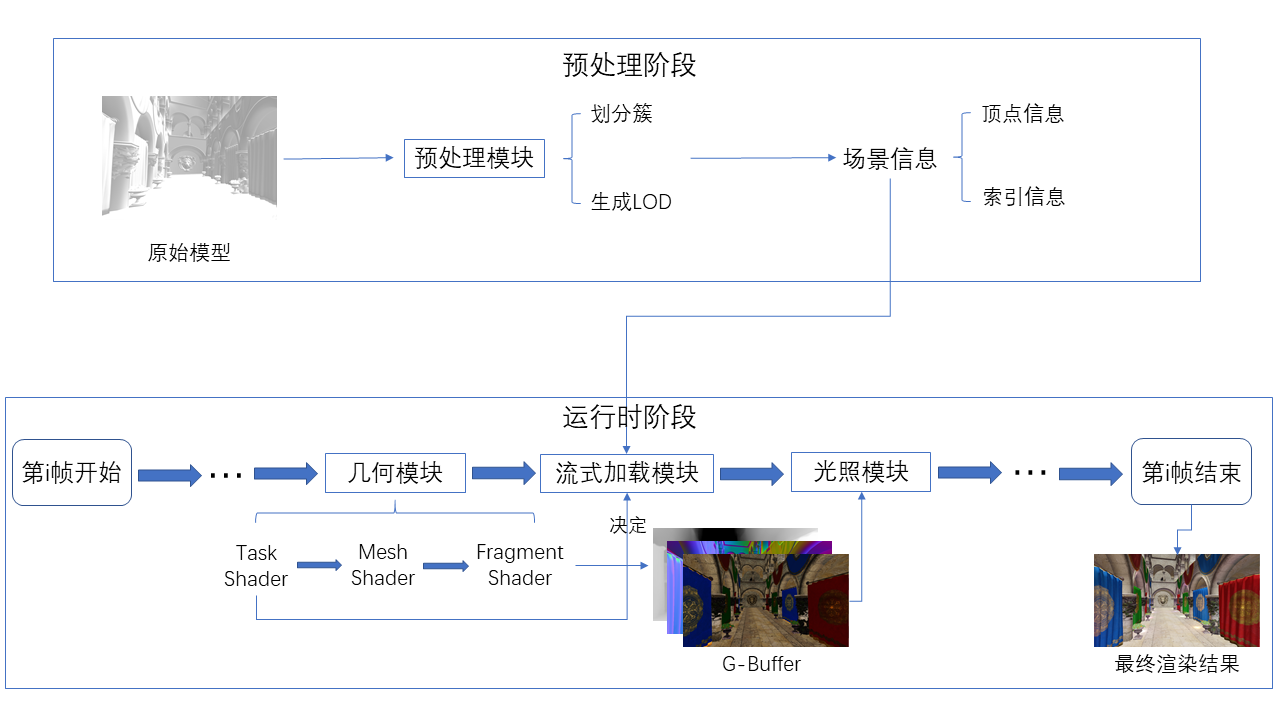
\includegraphics[width=\linewidth]{流程.png}
    \caption{\label{fig:流程}项目流程图}
\end{figure}

\par 综上所述,本项目在原有引擎渲染管线的基础上,主要负责对几何模块进行修改,新增流式加载模块,并在预处理阶段实现了模型划分成簇与生成 LOD 的功能。通过这些改进,原渲染管线的性能得到了显著优化,帧率明显提升,显存占用有所降低,同时保持了良好的画面保真度。

\section{基于簇的 GPU 驱动渲染管线}

\subsection{引言}

GPU 驱动的渲染管线是一种通过 GPU 完成大部分渲染任务的渲染架构,与传统的 CPU 驱动渲染管线相比,GPU 驱动渲染管线能够显著提高渲染效率,尤其在处理复杂或大规模场景时。其核心思想是将大量渲染计算和数据处理任务交给 GPU 执行,充分利用 GPU 强大的并行计算能力,从而加速渲染过程。

本项目除了流式加载模块中涉及到 CPU 与 GPU 之间的通信外,其余的渲染过程均在 GPU 上实现。与此同时,本项目引入了由任务着色器和网格着色器组成的新型渲染管线,代替了传统的计算着色器(Compute Shader)、顶点着色器(Vertex Shader)和几何着色器(Geometry Shader)的组合。网格着色器提出了“簇”这一新概念,通过将渲染单位组织为簇,显著提高了 GPU 批处理的性能\cite{Czubala2024}。

\subsection{基于簇的渲染}

基于簇的渲染最早由育碧(Ubisoft)在游戏《刺客信条:大革命》(Assassin's Creed Unity)中提出\cite{Ubisoft2015}。该方法将最小的剔除单元从传统的实例(instance)替换为簇,每个簇包含多个三角形,一个实例可以包含多个簇。通过这种更加细粒度的剔除方式,渲染引擎能够根据簇的可见性进行精确剔除。对于复杂模型,这种做法能减少需要绘制的多边形数量,从而显著降低渲染管线中的计算负担。

本项目在预处理阶段实现了簇的划分,并设计了基于簇的渲染管线,有效提高了渲染性能。

\subsubsection{簇的划分} \label{subsubsec:cluster division}

簇的划分是预处理阶段的关键步骤之一,本项目使用了第三方库 MeshOptimizer 来实现这一过程\cite{meshoptimizer}。MeshOptimizer 是一个高效的网格优化库,提供了各种优化算法,可以有效地对网格进行简化和划分,从而提高 GPU 渲染的性能。目前本项目只使用了该库的网格划分功能,在 \ref{subsec:LOD generation} 节中,本项目还会使用该库进行网格简化的操作。

在具体实践中,本项目规定每个簇最多由 64 个顶点 和 124 个三角形组成。这样的划分方式有助于平衡簇的大小和渲染效率\cite{Kubisch2018}。

\subsubsection{基于簇的剔除} \label{subsubsec:cluster culling}

基于簇的剔除是在任务着色器中进行的,本项目目前实现的剔除算法包括视锥剔除(Frustum Culling)和圆锥剔除(Cone Culling)。

其中,视锥剔除是判断模型是否在相机视野范围内的一种剔除方法。在预处理阶段,本项目提前计算了每个簇的包围球(Bounding Sphere),通过在运行时测试该包围球与视锥体(View Frustum)的关系,来判断该簇是否位于当前相机视野范围内。如果包围球完全在视锥体外,则该簇可以被剔除,避免不必要的渲染计算。

圆锥剔除则是通过将簇的可见性表达为一个圆锥形状来进行判断,圆锥的范围包含了簇的所有法线方向。具体而言,如果相机的视角方向与圆锥范围内的所有法线方向的点积均为负数,则说明该簇背对相机,可以整体剔除,不需要渲染。在预处理阶段,本项目同样计算了每个簇对应的圆锥信息,包括圆锥的顶点、主轴方向和定角等参数,这些信息可以直接用于运行时的剔除操作,大大提高了渲染效率。

\subsubsection{基于簇的网格着色器渲染管线}

网格着色器是基于簇的渲染工作流程中的关键步骤之一。在这一阶段,经过任务着色器剔除后的簇将被并行处理,网格着色器负责对簇进行坐标变换、图元组装等操作。每个簇包含多个顶点和图元,网格着色器能够高效地并行处理多个簇,显著减少传统渲染管线中的处理开销\cite{Santerre2020}。

经过网格着色器处理后,每个簇的顶点和索引信息将会被传递给片段着色器。片段着色器根据顶点的颜色、法线、纹理坐标等信息,计算每个像素的位置、法线和颜色等,用于后续的光照计算。

\subsection{测试分析报告}

本项目实现了簇的可视化功能,并在多个场景中进行了测试,如 \autoref{fig:Meshlet} 所示。可以看出,簇划分结果较为规整,能够较好地贴合几何结构,且不同场景下的可视化效果均展现出了良好的适应性和一致性。这为后续的基于簇的剔除与 LOD 管理提供了直观支撑。

% \begin{figure}[htbp]
%     \centering
%     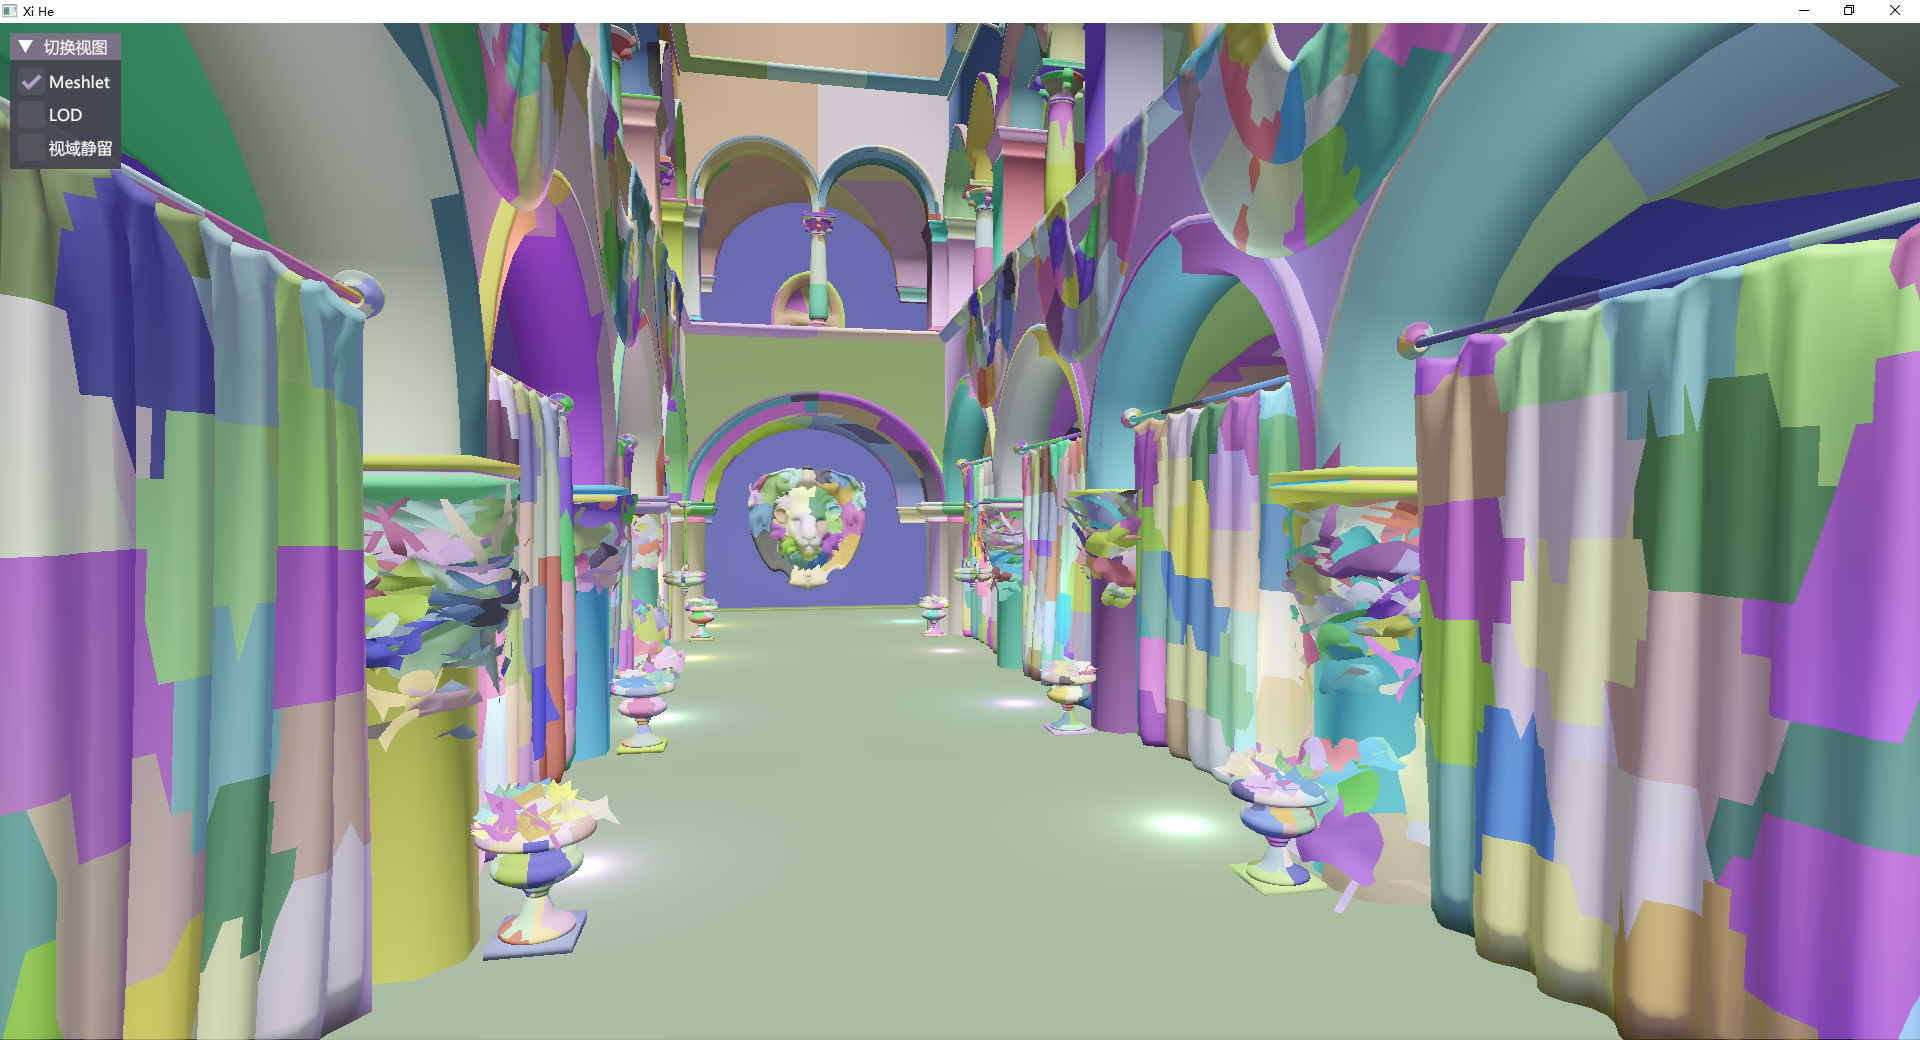
\includegraphics[width=\linewidth]{Meshlet.png}
%     \caption{\label{fig:Meshlet}簇的可视化效果图}
% \end{figure}

\begin{figure*}[htbp]
    \centering

    \begin{subfigure}[b]{0.48\linewidth}
        \centering
        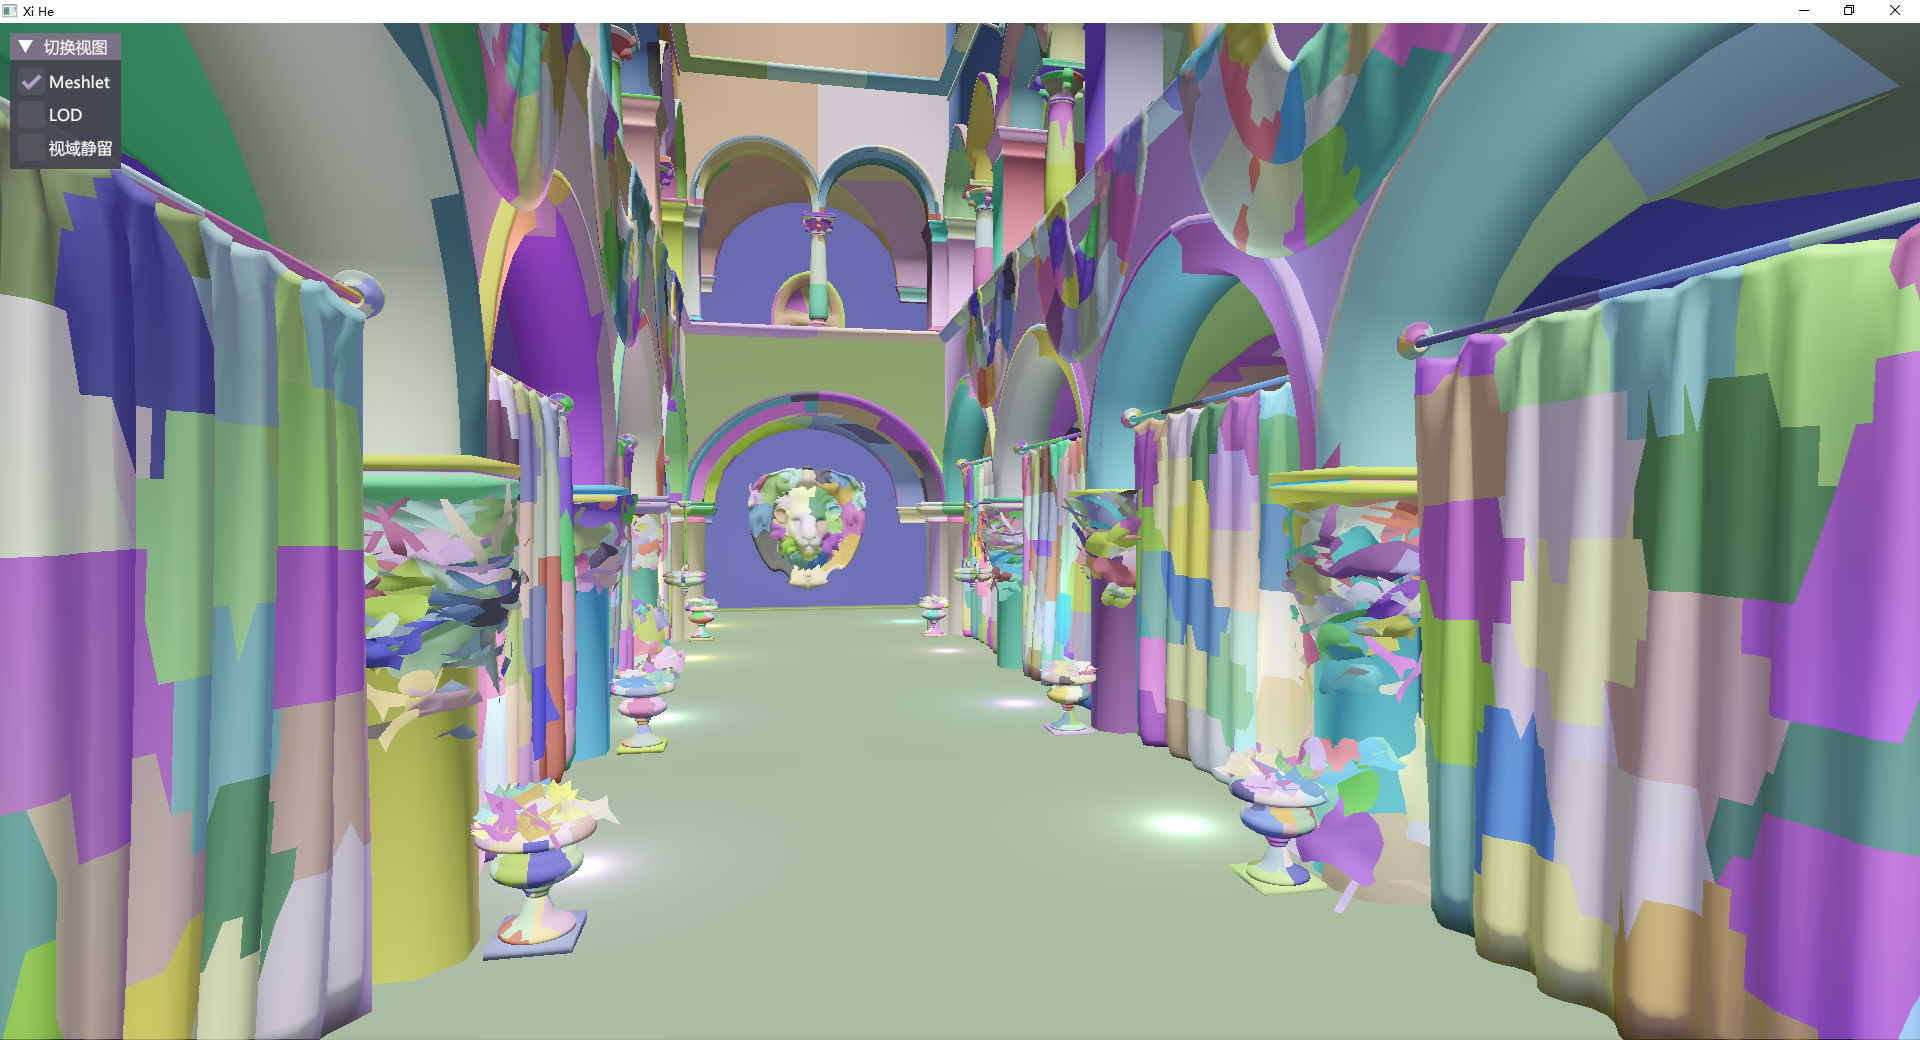
\includegraphics[width=\linewidth]{Meshlet.png}
        \caption{Sponza 场景}
    \end{subfigure}
    \hfill
    \begin{subfigure}[b]{0.48\linewidth}
        \centering
        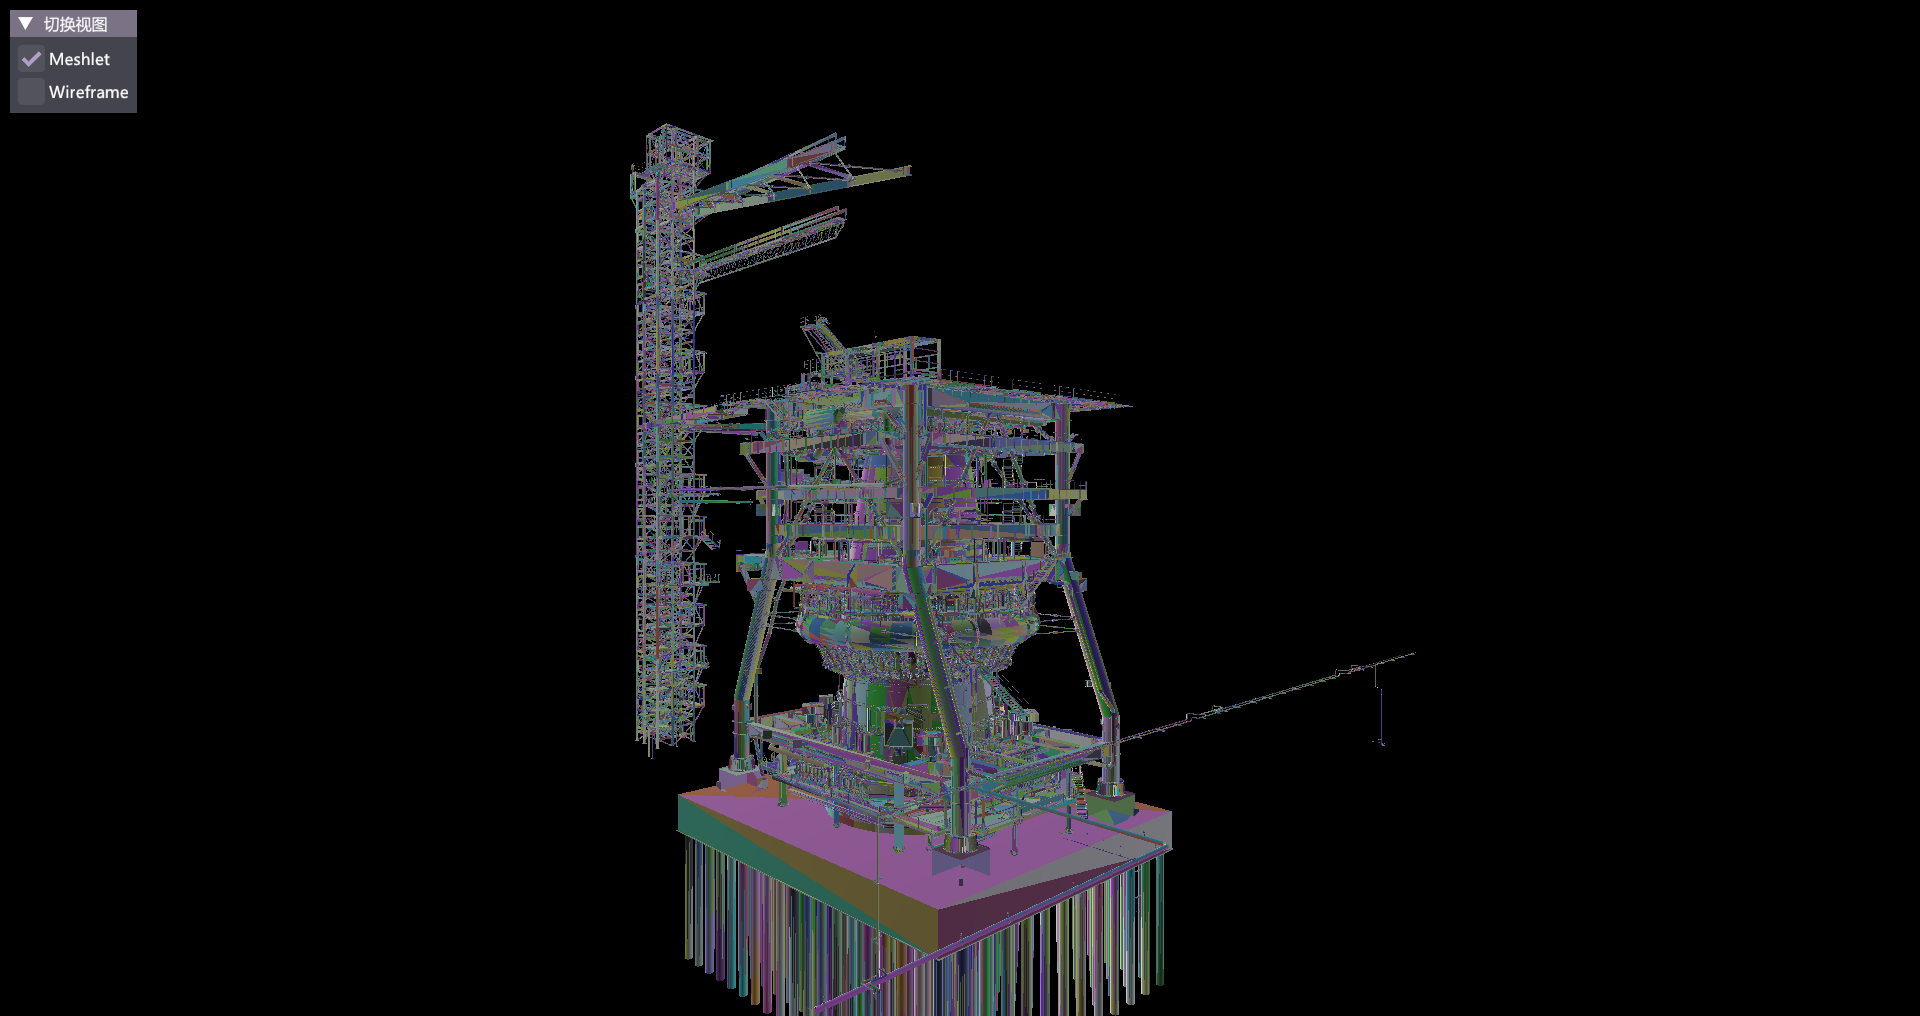
\includegraphics[width=\linewidth]{factory_meshlet.png}
        \caption{Factory 场景}
    \end{subfigure}

    \caption{簇的可视化效果图}
    \vspace{-0.2cm}
    \label{fig:Meshlet}
\end{figure*}

与此同时,本项目对 Factory 场景设置了固定相机轨迹进行测试,测量了不同剔除策略下的平均帧时间,以及 GPU 在裁剪阶段丢弃的平均图元数量。GPU 在裁剪阶段丢弃的图元数量越多,意味着处理了更多无效的几何数据,从而浪费了带宽和计算资源。具体测试结果见\autoref{tab:culling}。

\begin{table}[H]
    \caption{\label{tab:culling}不同剔除策略下的渲染性能测试结果}
    \begin{tabularx}{\linewidth}{|c|X<{\centering}|c|}
        \hline
        剔除策略 & GPU 在裁剪阶段丢弃的图元数 & 帧时间 \\ \hline
        不使用剔除 & 40713.9k & 240.7ms \\ \hline
        使用实例级剔除 & 40350.5k & 233.5ms \\ \hline
        使用视锥剔除 & 28557.5k & 147.9ms \\ \hline
        使用圆锥剔除 & 39249.1k & 230.7ms \\ \hline
        同时使用视锥剔除和圆锥剔除 & 27575.3k & 142.7ms \\ \hline
    \end{tabularx}
\end{table}

从表中数据可以看出,实例级的剔除对于工业大场景的性能提升有限,而基于簇的视锥剔除和圆锥剔除能够有效减少绘制三角形的数量。二者相结合的基于簇的剔除策略显著提升了渲染帧率,证明了基于簇的渲染方法在提高渲染效率方面的有效性。

\section{LOD 机制}

\subsection{引言}

LOD 是一种通过根据物体与视点的距离调整其细节程度的技术。当物体距离视点较远时,可以使用较粗糙的模型;而当物体距离视点较近时,则使用较精细的模型。这种技术能显在保证画面质量的同时,有效减少屏幕上绘制的三角形数量,提高渲染性能\cite{Deng2017}。而在本项目中,LOD 不仅用于提高渲染性能,还与流式加载结合,通过按需加载不同 LOD 的模型,进一步降低显存占用。

\subsection{LOD生成} \label{subsec:LOD generation}

LOD 生成部分参考了 Nanite 的核心思想,采用基于网格简化的 LOD 生成方法\cite{Jensen2023},整体过程大致可以分为以下几步\cite{Xavier2024}:

\newcommand{\stepref}[1]{\textbf{Step~\ref{#1}}}

\begin{enumerate}
    \item 将初始模型划分为簇;
    \item 根据簇之间的连接性,将簇组织成簇组(cluster group),每个簇组最多包含 16 个簇;
    \item 对每个簇组进行独立简化,确保每个簇组的边界完整,从而避免不同 LOD 之间出现裂缝;
    \item 将简化后的簇组重新划分为新的簇;
    \item 如果新的簇数量仍然过多,则返回步骤 2 进行进一步简化;否则,结束生成过程。
\end{enumerate}

其中,步骤 1 已经在 \ref{subsubsec:cluster division} 节中,通过使用 MeshOptimizer 库得到了有效解决。步骤 4 也可以采用类似的方法来处理。

在步骤 2 中,本项目将已生成的簇进一步划分为若干簇组。理想情况下,簇组之间的共享边应尽可能少,以最大程度减少后续步骤中因跨组操作而需锁定的顶点数量。该问题可等效视为串行图划分(Serial Graph Partitioning)问题,该问题可采用 METIS 等图划分库进行高效求解\cite{METIS}。

而对于每个簇组,将使用 MeshOptimizer 库对其进行锁定边界的简化,即步骤 3。简化结束后,MeshOptimizer 库会返回一个误差值,用以表示简化后的簇组与原簇组的相对误差。该误差值将在 \ref{subsec:run-time lod select} 节中用于运行时的 LOD 选择。

为了确保简化过程能够顺利进行,还需要将空间距离较近的顶点进行合并。这是因为,对于拓扑结构不一致或存在大量缝隙(seam)的网格时,简化器可能会“卡住”,无法有效地简化网格。顶点合并能够有效改善这一情况,促进整个简化过程。

为了高效查询每个顶点的最近邻,本项目使用 K-D 树对顶点进行管理\cite{bentley1975}。K-D 树的构建时间复杂度一般为 $O(N\log N)$,单次查询的时间复杂度为 $O(\log N)$。相比于枚举算法的 $O(N^2)$ 时间复杂度,K-D 树的效率更高,满足本项目对预处理时间复杂度的需求。

此外,为避免顶点合并后模型的视觉差异过大,本项目在顶点合并时不仅考虑顶点在空间上的距离,还将纹理坐标、法向量等因素考虑在内。

为进一步提高预处理速度,本项目引入 oneTBB 库对整个预处理过程进行多线程加速\cite{oneTBB},重点对顶点合并等易成为瓶颈的步骤进行了优化。

完成以上所有步骤后,不同 LOD 等级的簇将构成一个有向无环图(DAG),如\autoref{fig:DAG}所示\cite{WangXi2022}。该图中,每个节点表示一个簇,每个节点可能有多个父节点,父节点是由子节点简化得来的。被矩形框住的节点同属一个簇组。在随后的运行时阶段,本项目将基于该有向无环图来进行 LOD 选择。

\begin{figure}[ht]
    \centering
    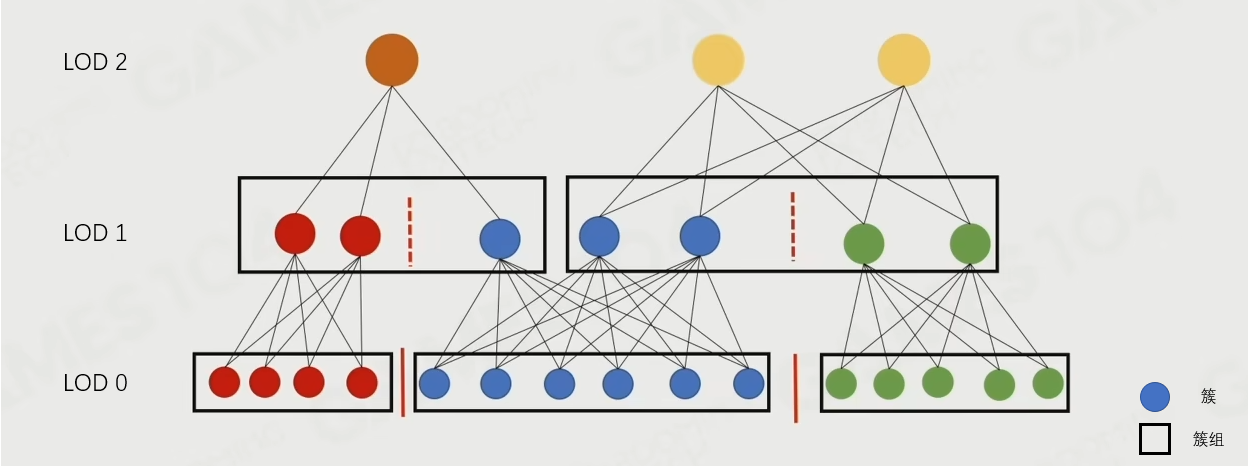
\includegraphics[width=\linewidth]{DAG.png}
    \caption{\label{fig:DAG}LOD的DAG示意图}
\end{figure}

\subsection{运行时 LOD 选择} \label{subsec:run-time lod select}

\par 为了在运行时进行 LOD 选择,必须对\autoref{fig:DAG}中的有向无环图进行遍历。而传统的遍历方法缺乏并发性,无法直接在 GPU 上执行。为了实现并行,本项目对每个节点(簇)独立进行 LOD 选择。为此,需要在 LOD 生成阶段预先维护每个节点(簇)所在簇组的误差值、包围球,以及其父节点所在簇组的误差值和包围球信息\cite{WangQian2016}。由于每个节点可能有多个父节点,且这些父节点可能属于不同的簇组,因此在维护父节点的误差值和包围球时,通常取其中的最大值。

在运行时,基于这些预计算的数据,本项目将计算每个节点自身在屏幕空间上的误差 $cluster\_error$,以及其父节点在屏幕空间上的误差 $parent\_error$。这两者的值由节点自身的误差以及其包围球在屏幕空间上的投影大小决定。与此同时,本项目设置了一个阈值 $lod\_threshold$,当且仅当 $cluster\_error < lod\_threshold$ 且 $parent\_error \geq lod\_threshold$ 时,该节点(簇)才有可能被绘制。这种可见性判定机制确保了渲染时的层级互斥性:当某个子节点满足条件被绘制时,其所有父节点必然不符合渲染条件,因而不会被同时绘制。

这种基于簇的 LOD 选择方法兼具并行化优势,可与基于簇的剔除(参见\ref{subsubsec:cluster culling})在任务着色器中同步完成,无需引入额外渲染通道。该方案显著降低了实现复杂度,同时提升了整体渲染效率。

\subsection{测试分析报告}

本项目首先基于 Sponza 场景的局部模型进行 LOD 生成测试,效果如\autoref{fig:LOD generation}所示。图中上方展示渲染结果,下方呈现对应的网格簇分布可视化。各 LOD 层级对应的顶点数、三角形数及簇数统计详见\autoref{tab:LOD}。

% \begin{figure}[!htb]
%     \centering
%     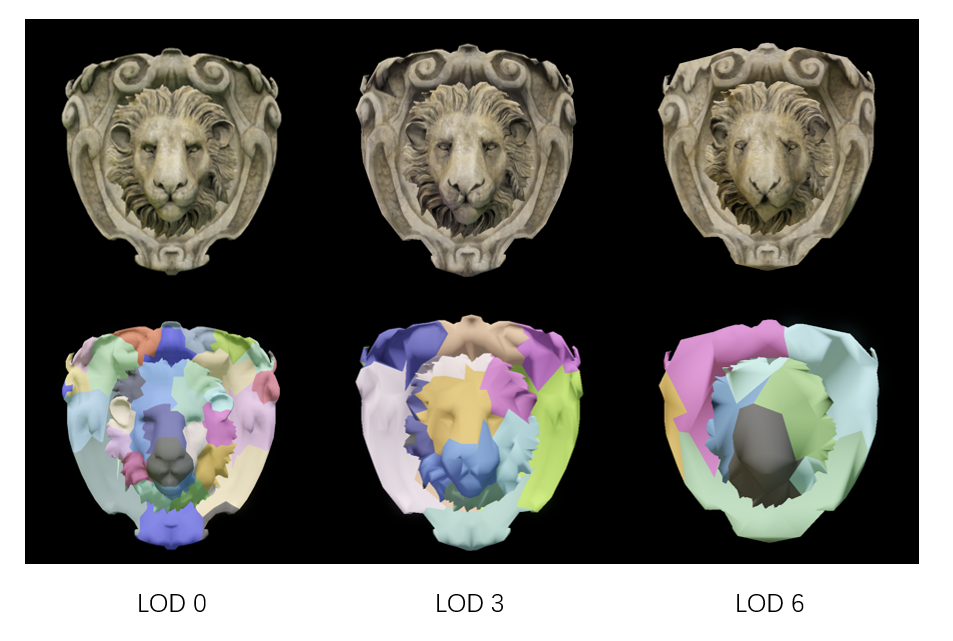
\includegraphics[width=\linewidth]{LOD生成.png}
%     \caption{\label{fig:LOD generation}各级 LOD 的生成效果图}
% \end{figure}

\begin{figure*}[h]
    \centering
    % 第一列(LOD 0)
    \begin{subfigure}[t]{0.32\linewidth}
        \centering
        
\includegraphics[width=\linewidth,height=1.6in,keepaspectratio]{tiger0.png}\\
        \vspace{0.1cm}
        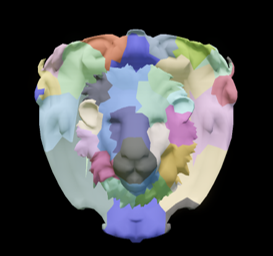
\includegraphics[width=\linewidth,height=1.6in,keepaspectratio]{tiger0_meshlet.png}
        \caption{LOD 0}
    \end{subfigure}%
    \hfill
    % 第二列(LOD 3)
    \begin{subfigure}[t]{0.32\linewidth}
        \centering
        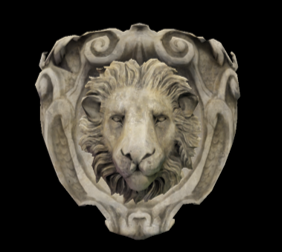
\includegraphics[width=\linewidth,height=1.6in,keepaspectratio]{tiger3.png}\\
        \vspace{0.1cm}
        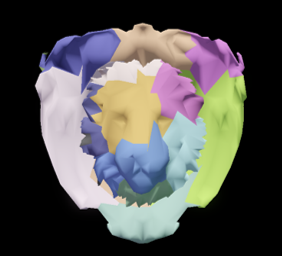
\includegraphics[width=\linewidth,height=1.6in,keepaspectratio]{tiger3_meshlet.png}
        \caption{LOD 3}
    \end{subfigure}%
    \hfill
    % 第三列(LOD 6)
    \begin{subfigure}[t]{0.32\linewidth}
        \centering
        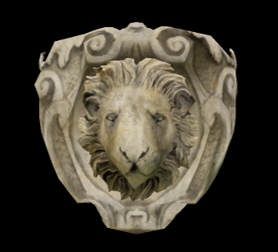
\includegraphics[width=\linewidth,height=1.6in,keepaspectratio]{tiger6.png}\\
        \vspace{0.1cm}
        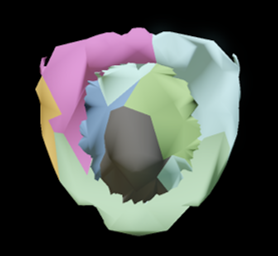
\includegraphics[width=\linewidth,height=1.6in,keepaspectratio]{tiger6_meshlet.png}
        \caption{LOD 6}
    \end{subfigure}
    \caption{各级 LOD 生成效果对比图}
    \label{fig:LOD generation}
\end{figure*}

\begin{table}[H]
    \caption{\label{tab:LOD}各级 LOD 对应的顶点数、三角形数和簇数}
    \begin{tabularx}{\linewidth}{|X<{\centering}|X<{\centering}|X<{\centering}|X<{\centering}|}
        \hline
        LOD级别 & 顶点数 & 三角数 & 簇数 \\ \hline
        LOD 0 & 5032 & 7128 & 80 \\ \hline
        LOD 3 & 2223 & 2997 & 36 \\ \hline
        LOD 6 & 1108 & 1264 & 18 \\ \hline
    \end{tabularx}
\end{table}

从上述结果可以看出,LOD 生成的核心功能基本实现,随着 LOD 级别的增大,顶点数、三角形数和簇数都有了明显下降,效果良好。

本项目对运行时 LOD 选择机制进行了验证测试,通过远景、中景和近景三个典型视距下的渲染效果对比,展示了 LOD 系统的实际表现(见\autoref{fig:LOD select})。图中第一行为原始场景渲染结果,第二行为应用 LOD 后的场景,第三行通过色彩编码可视化 LOD 层级分布,其中蓝色表示最高精度的 LOD 0 ,紫色代表中间层级,红色则对应最简化的 LOD。

\begin{figure*}[h]
    \centering
    % 第一列(远景)
    \begin{subfigure}[b]{0.32\linewidth}
        \centering
        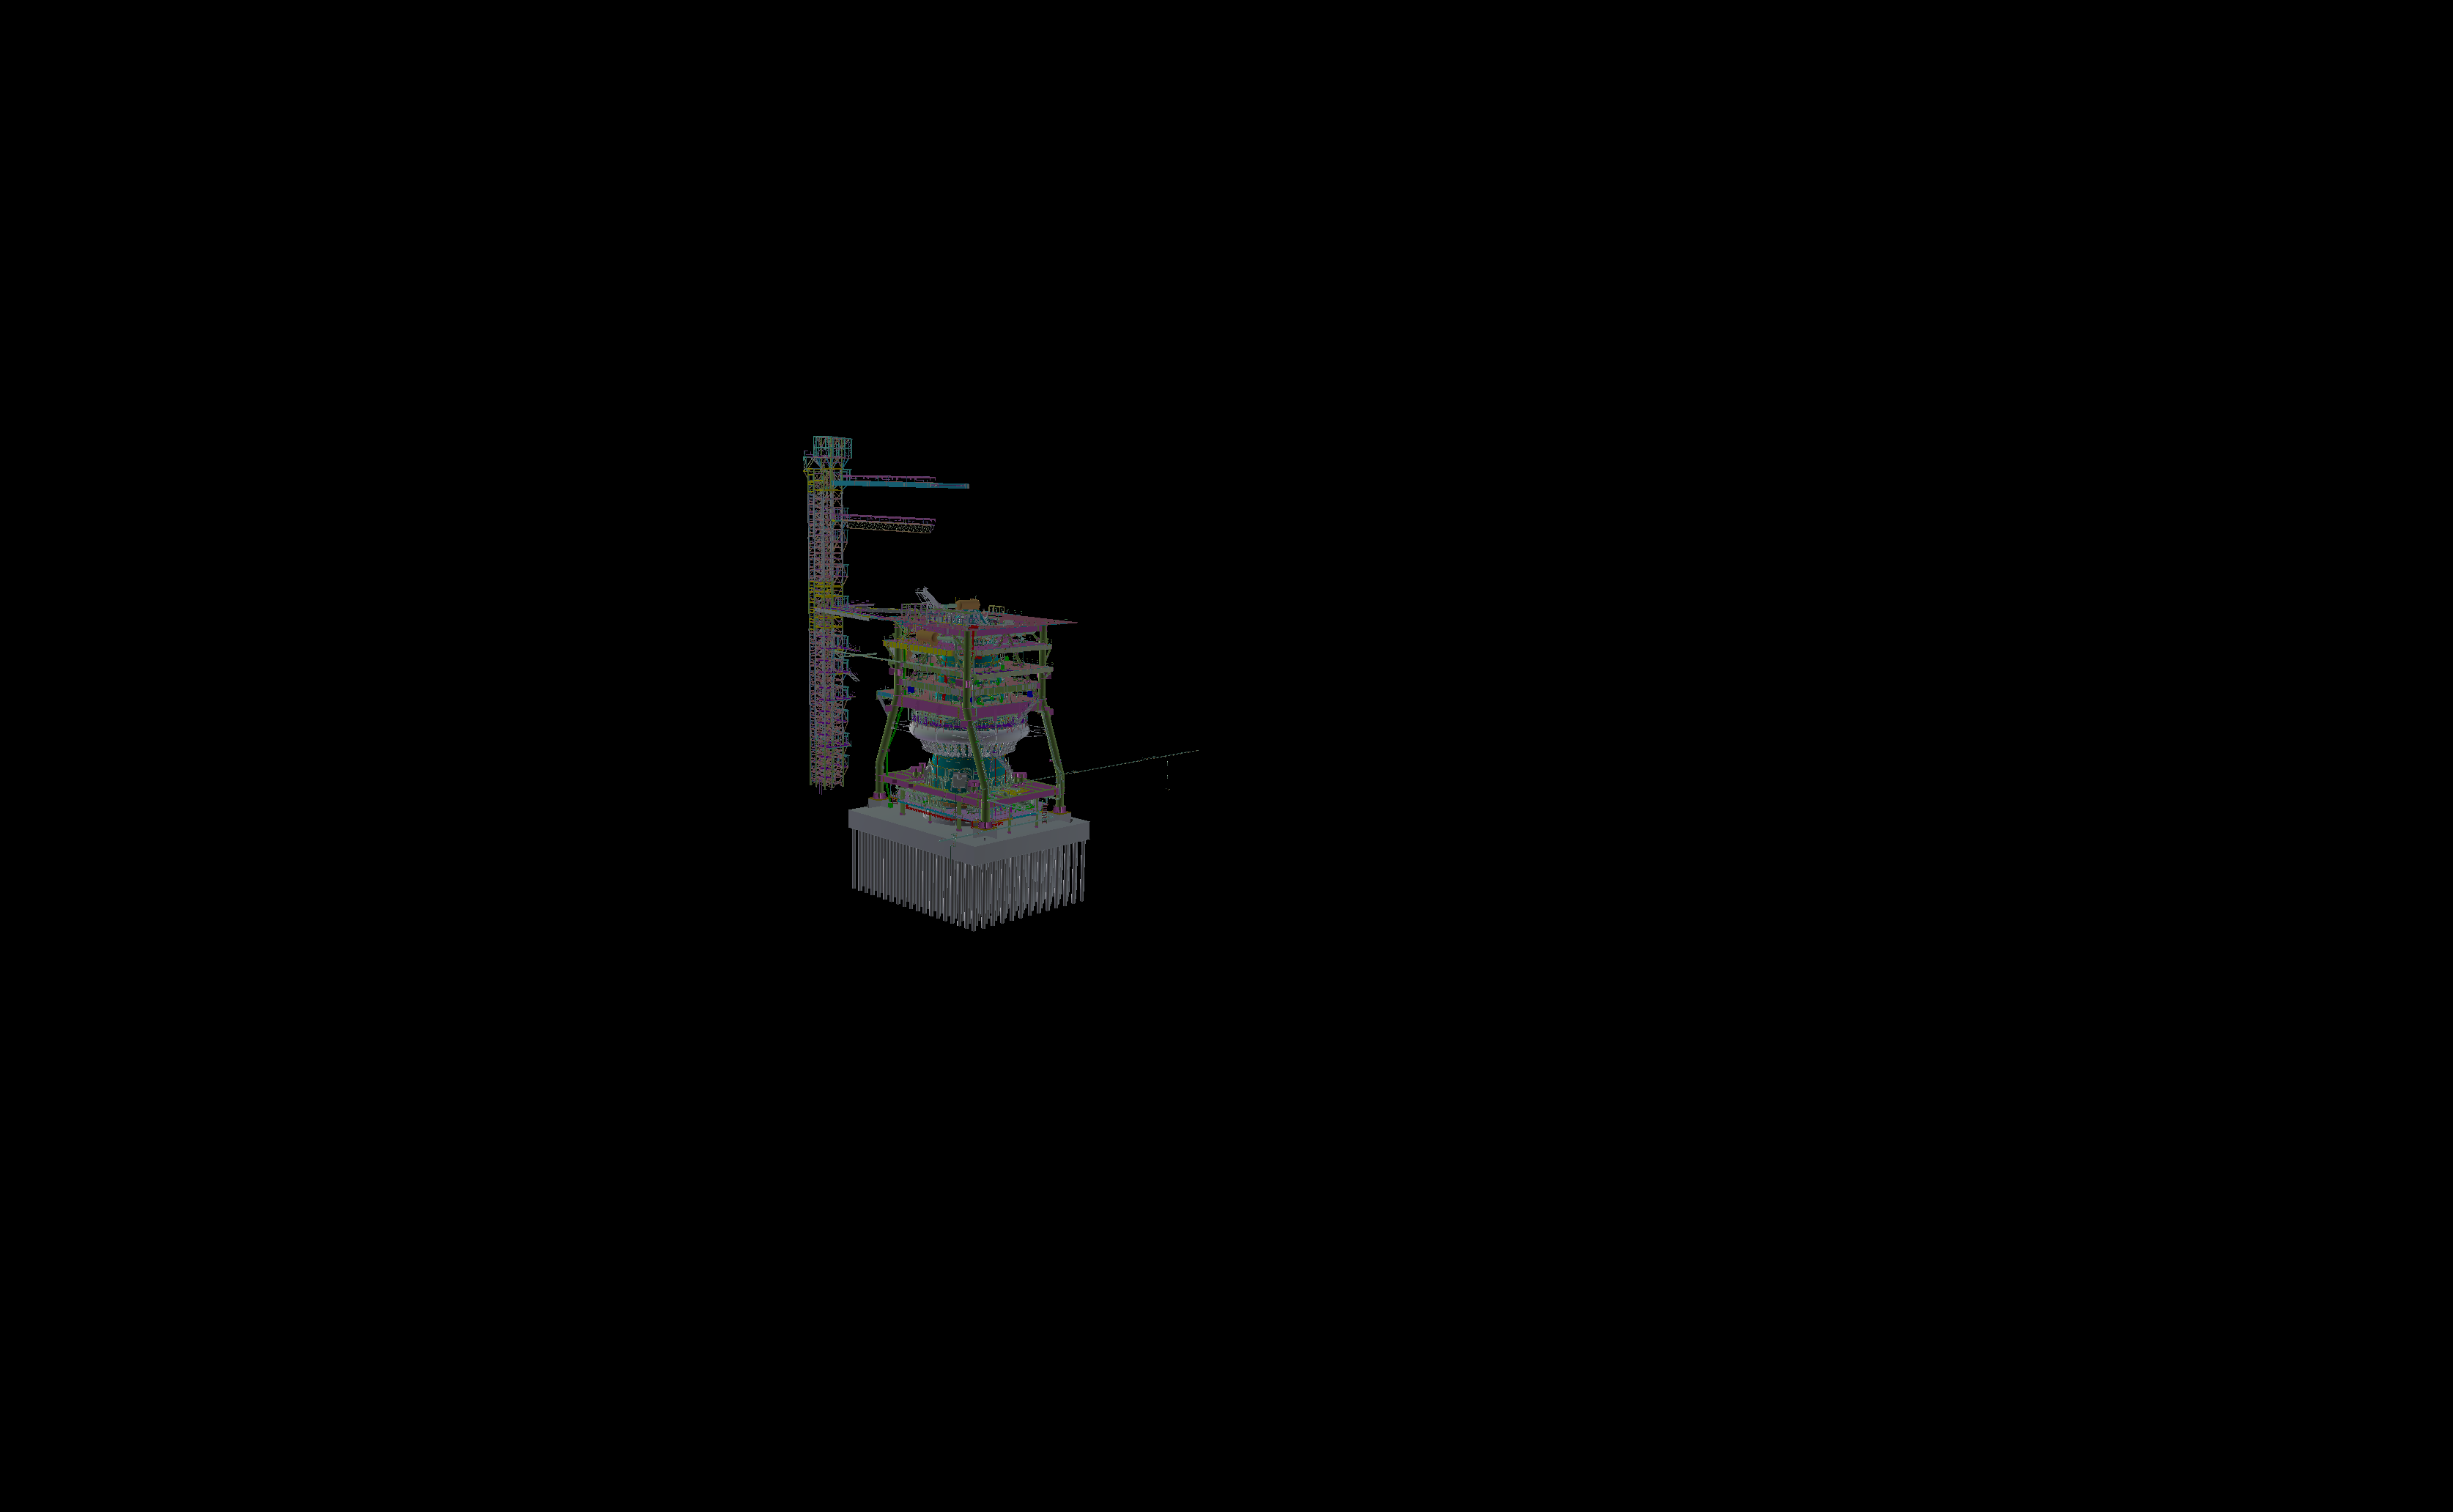
\includegraphics[width=\linewidth,height=1.6in,keepaspectratio]{远LOD0.png}\\
        \vspace{0.1cm}
        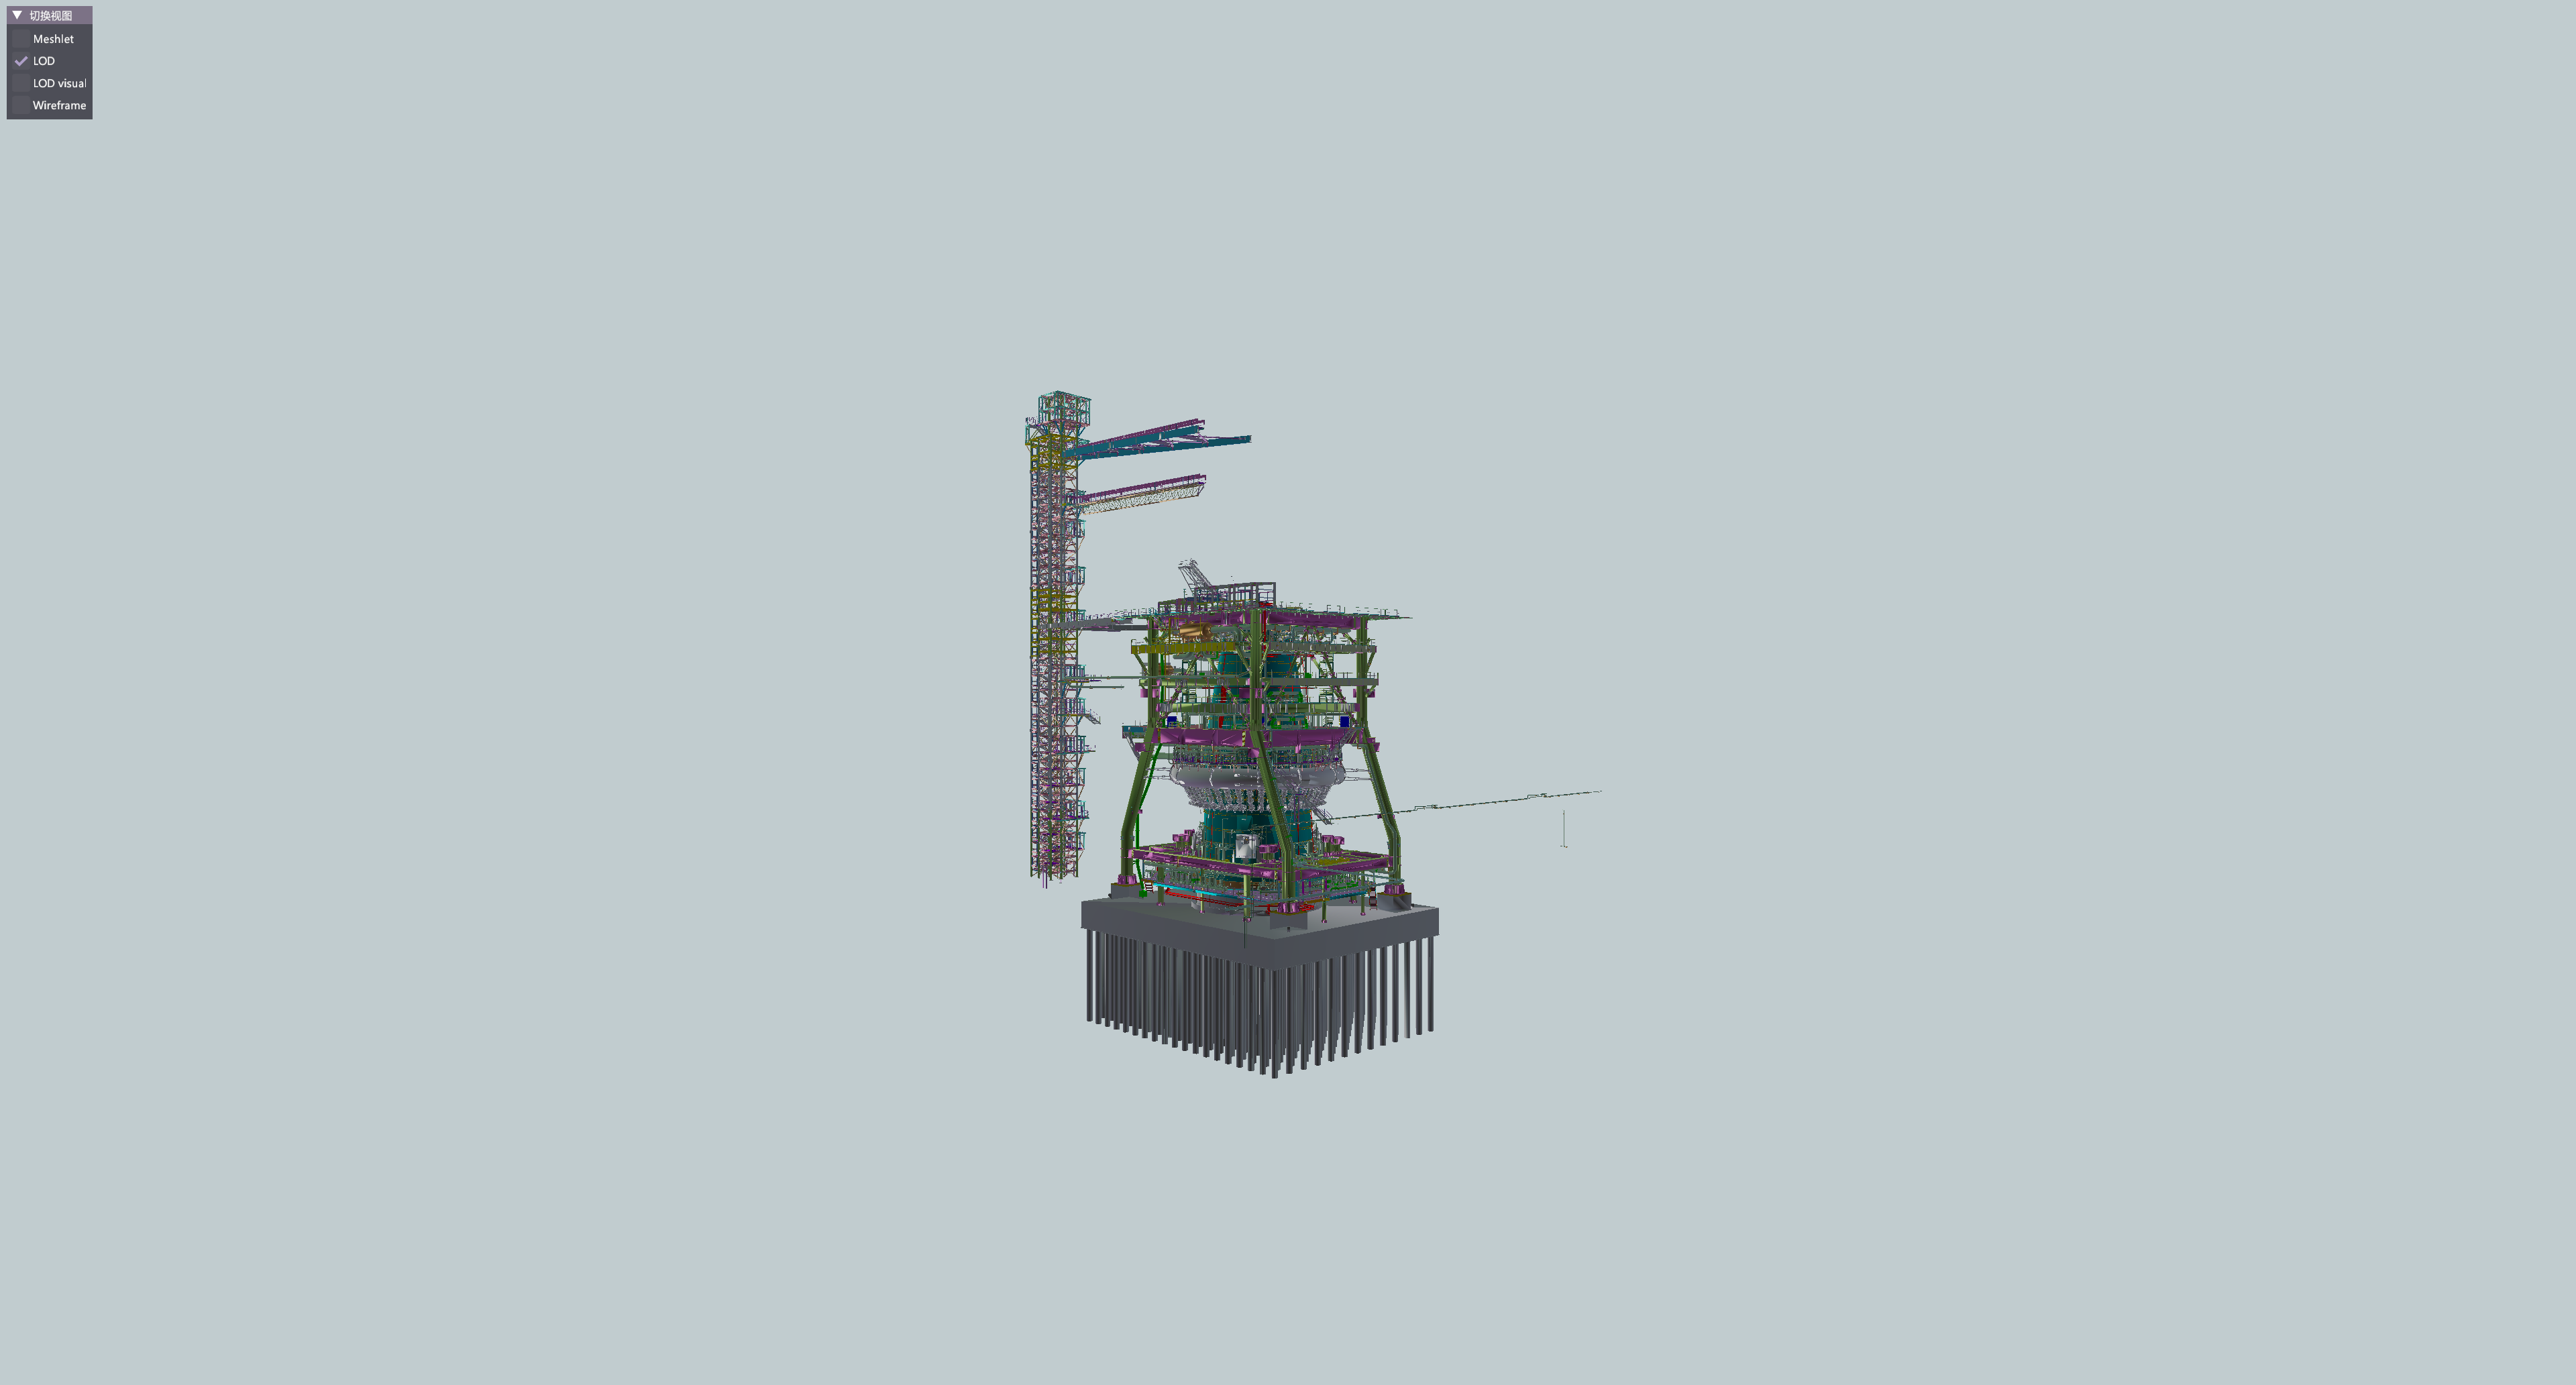
\includegraphics[width=\linewidth,height=1.6in,keepaspectratio]{远LOD.png}\\
        \vspace{0.1cm}
        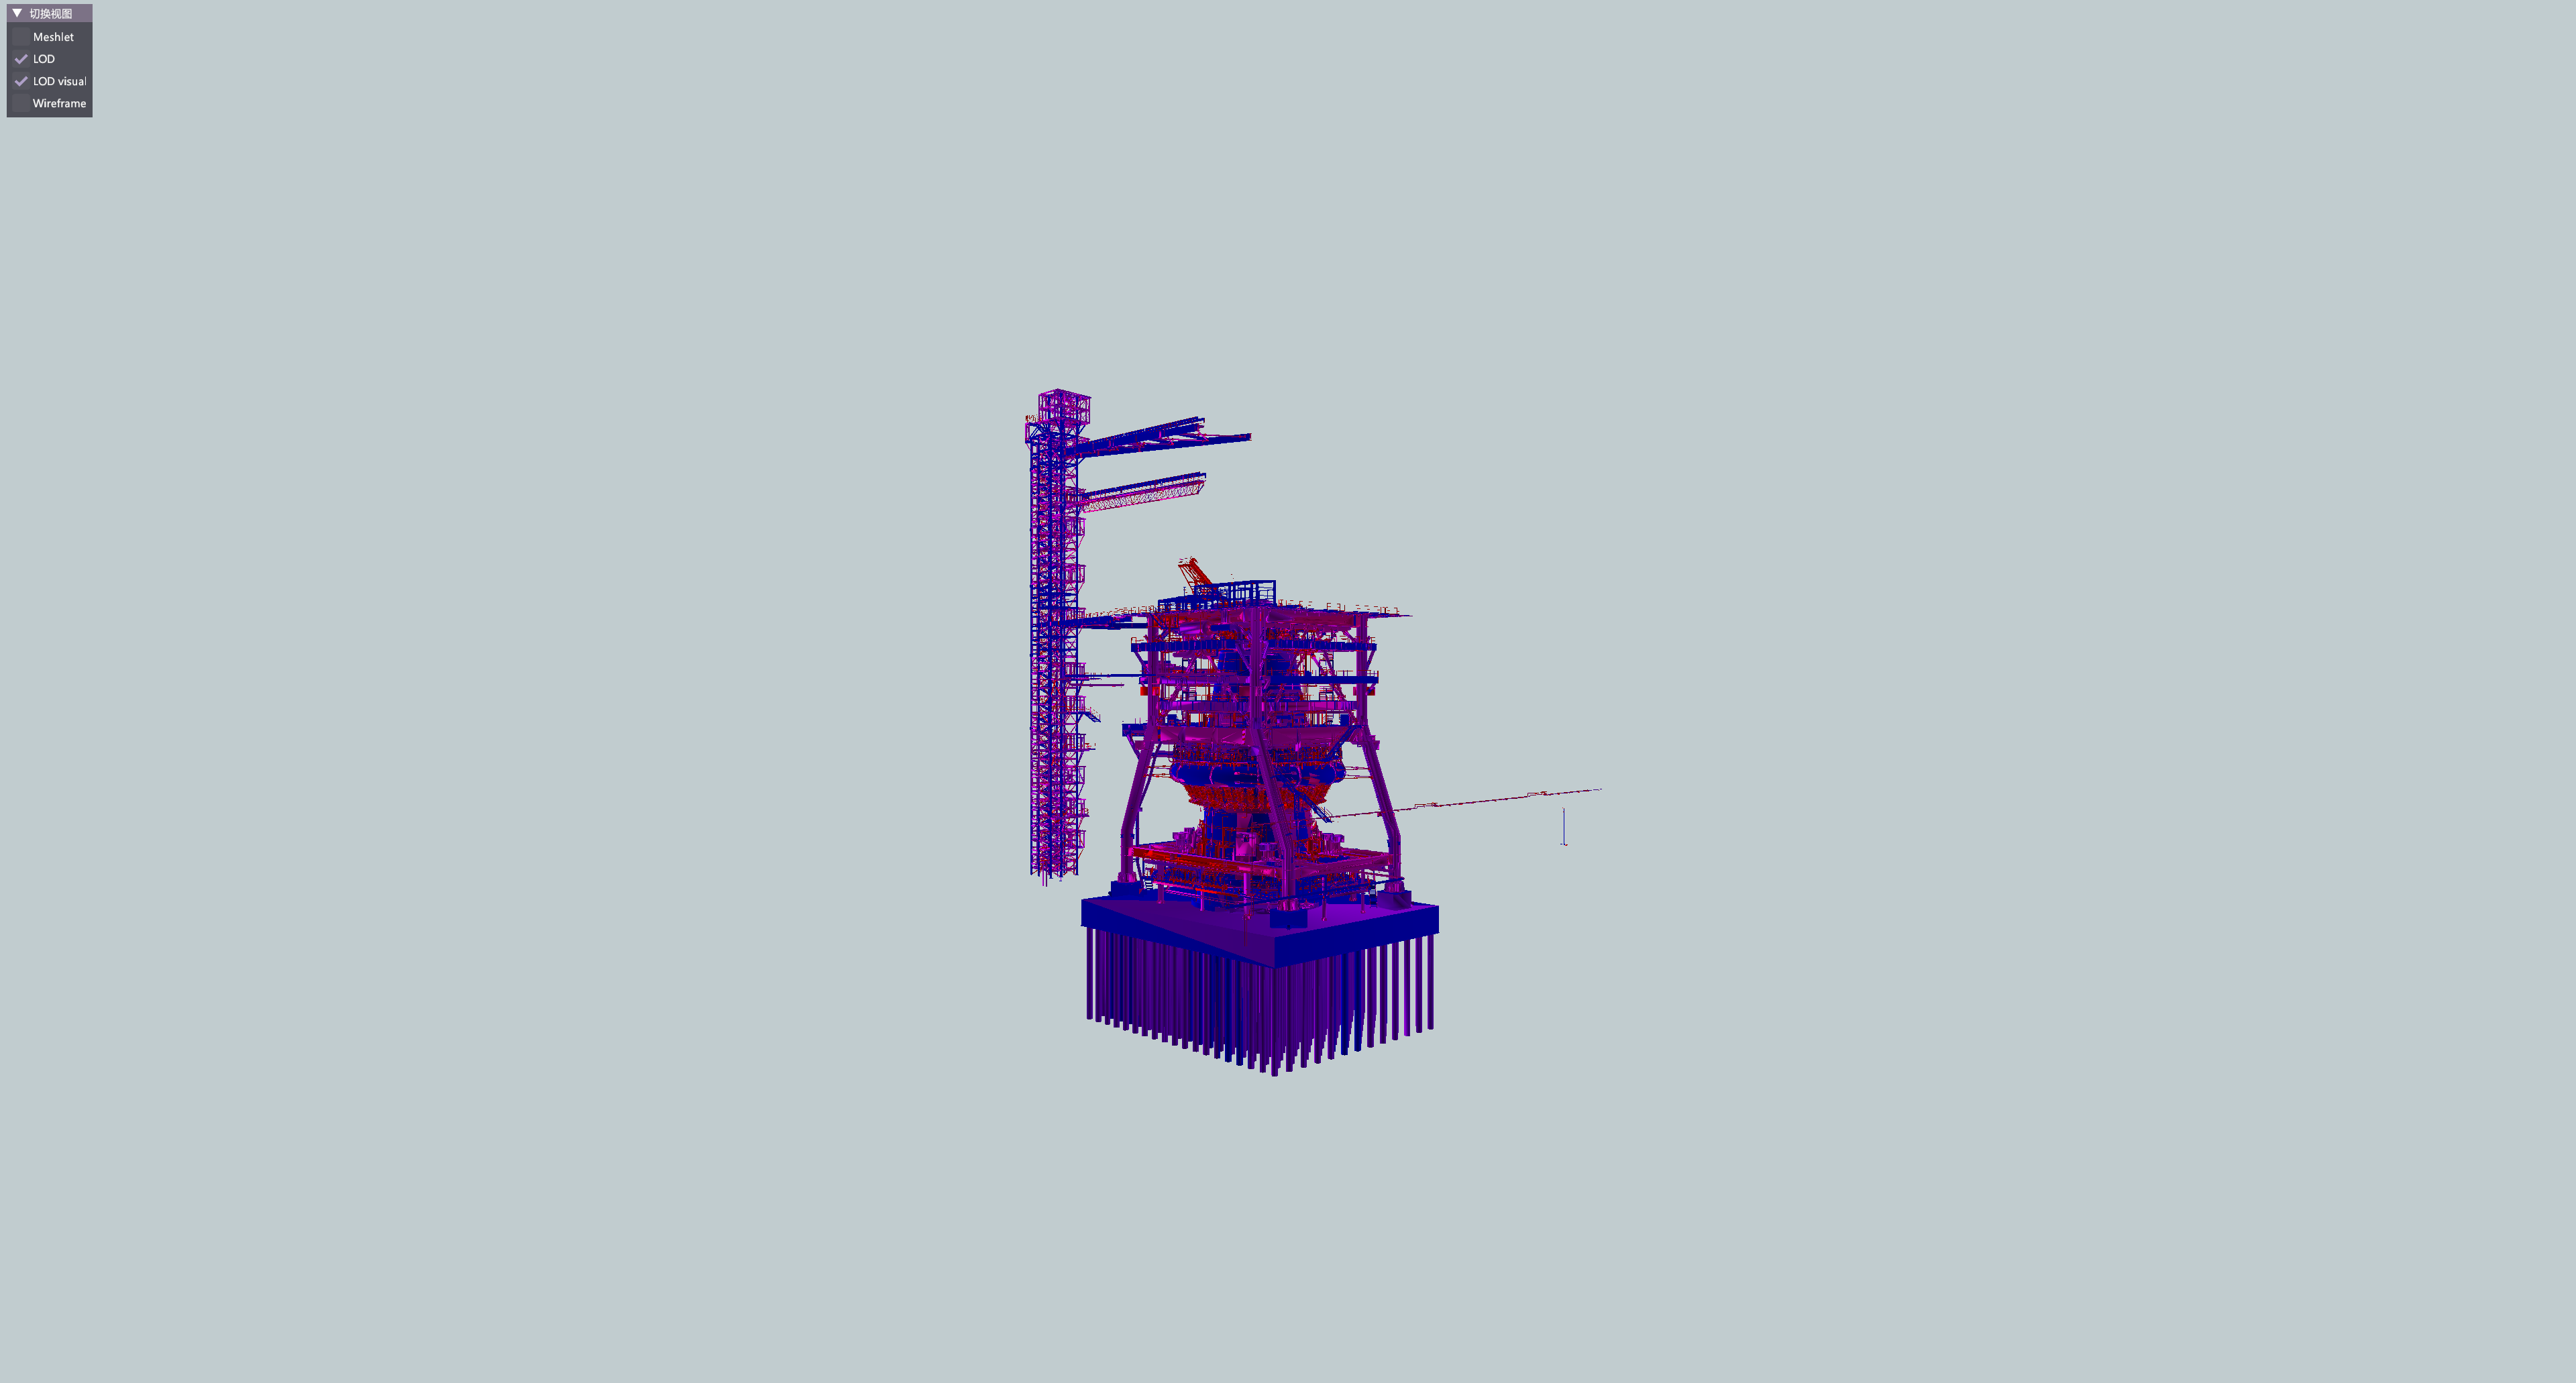
\includegraphics[width=\linewidth,height=1.6in,keepaspectratio]{远LODv.png}
        \caption{远景}
    \end{subfigure}%
    \hfill % 确保子图之间有空隙
    % 第二列(中景)
    \begin{subfigure}[b]{0.32\linewidth}
        \centering
        \includegraphics[width=\linewidth,height=1.6in,keepaspectratio]{中LOD0.png}\\
        \vspace{0.1cm}
        \includegraphics[width=\linewidth,height=1.6in,keepaspectratio]{中LOD.png}\\
        \vspace{0.1cm}
        \includegraphics[width=\linewidth,height=1.6in,keepaspectratio]{中LODv.png}
        \caption{中景}
    \end{subfigure}%
    \hfill % 确保子图之间有空隙
    % 第三列(近景)
    \begin{subfigure}[b]{0.32\linewidth}
        \centering
        \includegraphics[width=\linewidth,height=1.6in,keepaspectratio]{近LOD0.png}\\
        \vspace{0.1cm}
        \includegraphics[width=\linewidth,height=1.6in,keepaspectratio]{近LOD.png}\\
        \vspace{0.1cm}
        \includegraphics[width=\linewidth,height=1.6in,keepaspectratio]{近LODv.png}
        \caption{近景}
    \end{subfigure}
    \caption{LOD 选择策略在不同视距下的应用效果}
    \label{fig:LOD select}
\end{figure*}

测试结果表明,本项目的 LOD 选择机制具有明确的视距相关性:在远景下,系统倾向于选择最粗糙的 LOD(红色区域);在中景下,中等细节层次的 LOD(紫色和蓝色区域)成为主导;在近景下,画面上基本采用最精细的 LOD(蓝色区域)。这种与视距高度匹配的 LOD 分布特征,充分验证了本系统 LOD 选择算法的合理性与实用性。

\section{流式加载} \label{sec:streaming}

\subsection{引言}

流式加载是一种基于视域需求的动态资源加载技术,其优势在于能够显著降低显存占用。与传统的预加载模式相比,该技术有效避免了一次性加载大规模数据带来的显存压力\cite{sahm2004}。

本项目的流式加载系统实现了双重优化机制:首先,通过视域剔除技术,仅加载当前可见范围内的场景数据\cite{CohenOr2003};其次,结合 LOD 技术,对远距离物体仅加载简化层级的模型数据。

在预处理阶段,本项目将场景数据分页存储在 CPU 内存中;在运行时阶段,通过智能调度机制,将需要的数据页传输至 GPU 显存。这种设计在保证渲染性能和画面质量的前提下,实现了显存利用率的最大化。

\subsection{场景数据的存储}

在预处理阶段,本项目以簇组为单位对场景数据进行存储。主要原因是在任务着色器中,剔除计算与 LOD 选择均以簇组为单位。对于某一个簇组,要么整体渲染、要么整体跳过。在这种情况下,以簇组为单位存储数据具备以下优势:

\begin{enumerate}
    \item 降低 CPU 内存占用:若以簇为单位存储数据,由于簇与簇之间存在大量公共顶点,重复存储会导致内存占用大幅膨胀,而以簇组为单位能有效缓解该情况;
    \item 提高显存利用率:簇组内顶点与索引数据的紧凑布局有助于提高显存利用率,在有限的显存中存储更多有效几何信息;
    \item 提升访问效率:簇组结构具备更好的空间局部性\cite{MCCOOL2012},有助于提高缓存命中率,降低页表管理与数据交换的运行时开销。
\end{enumerate}

\subsection{动态加载}

在任务着色器中,所有簇组需依次进行剔除测试和 LOD 选择,只有通过测试的簇组的几何数据会被加载至 GPU 显存。因此,任务着色器需记录所有通过测试的簇组所对应的数据页编号,并将其传递给 CPU。CPU 利用页表(Page Table)对数据页进行统一管理,并借助 Vulkan 提供的稀疏资源机制,实现数据页的动态绑定,从而高效地完成资源调度。

\subsubsection{页表管理}

在本项目中,页表的容量和数据页的大小均为固定值,每个页表条目对应一个显存页。当 GPU 请求加载新的数据页时,CPU 首先检查该数据页是否已在页表中。若在,则不需要执行任何操作;若不在,则需在页表中寻找空闲条目,或选择一个当前帧未使用的数据页进行替换。页表结构如\autoref{fig:page table}所示。

\begin{figure}[htbp]
\centering
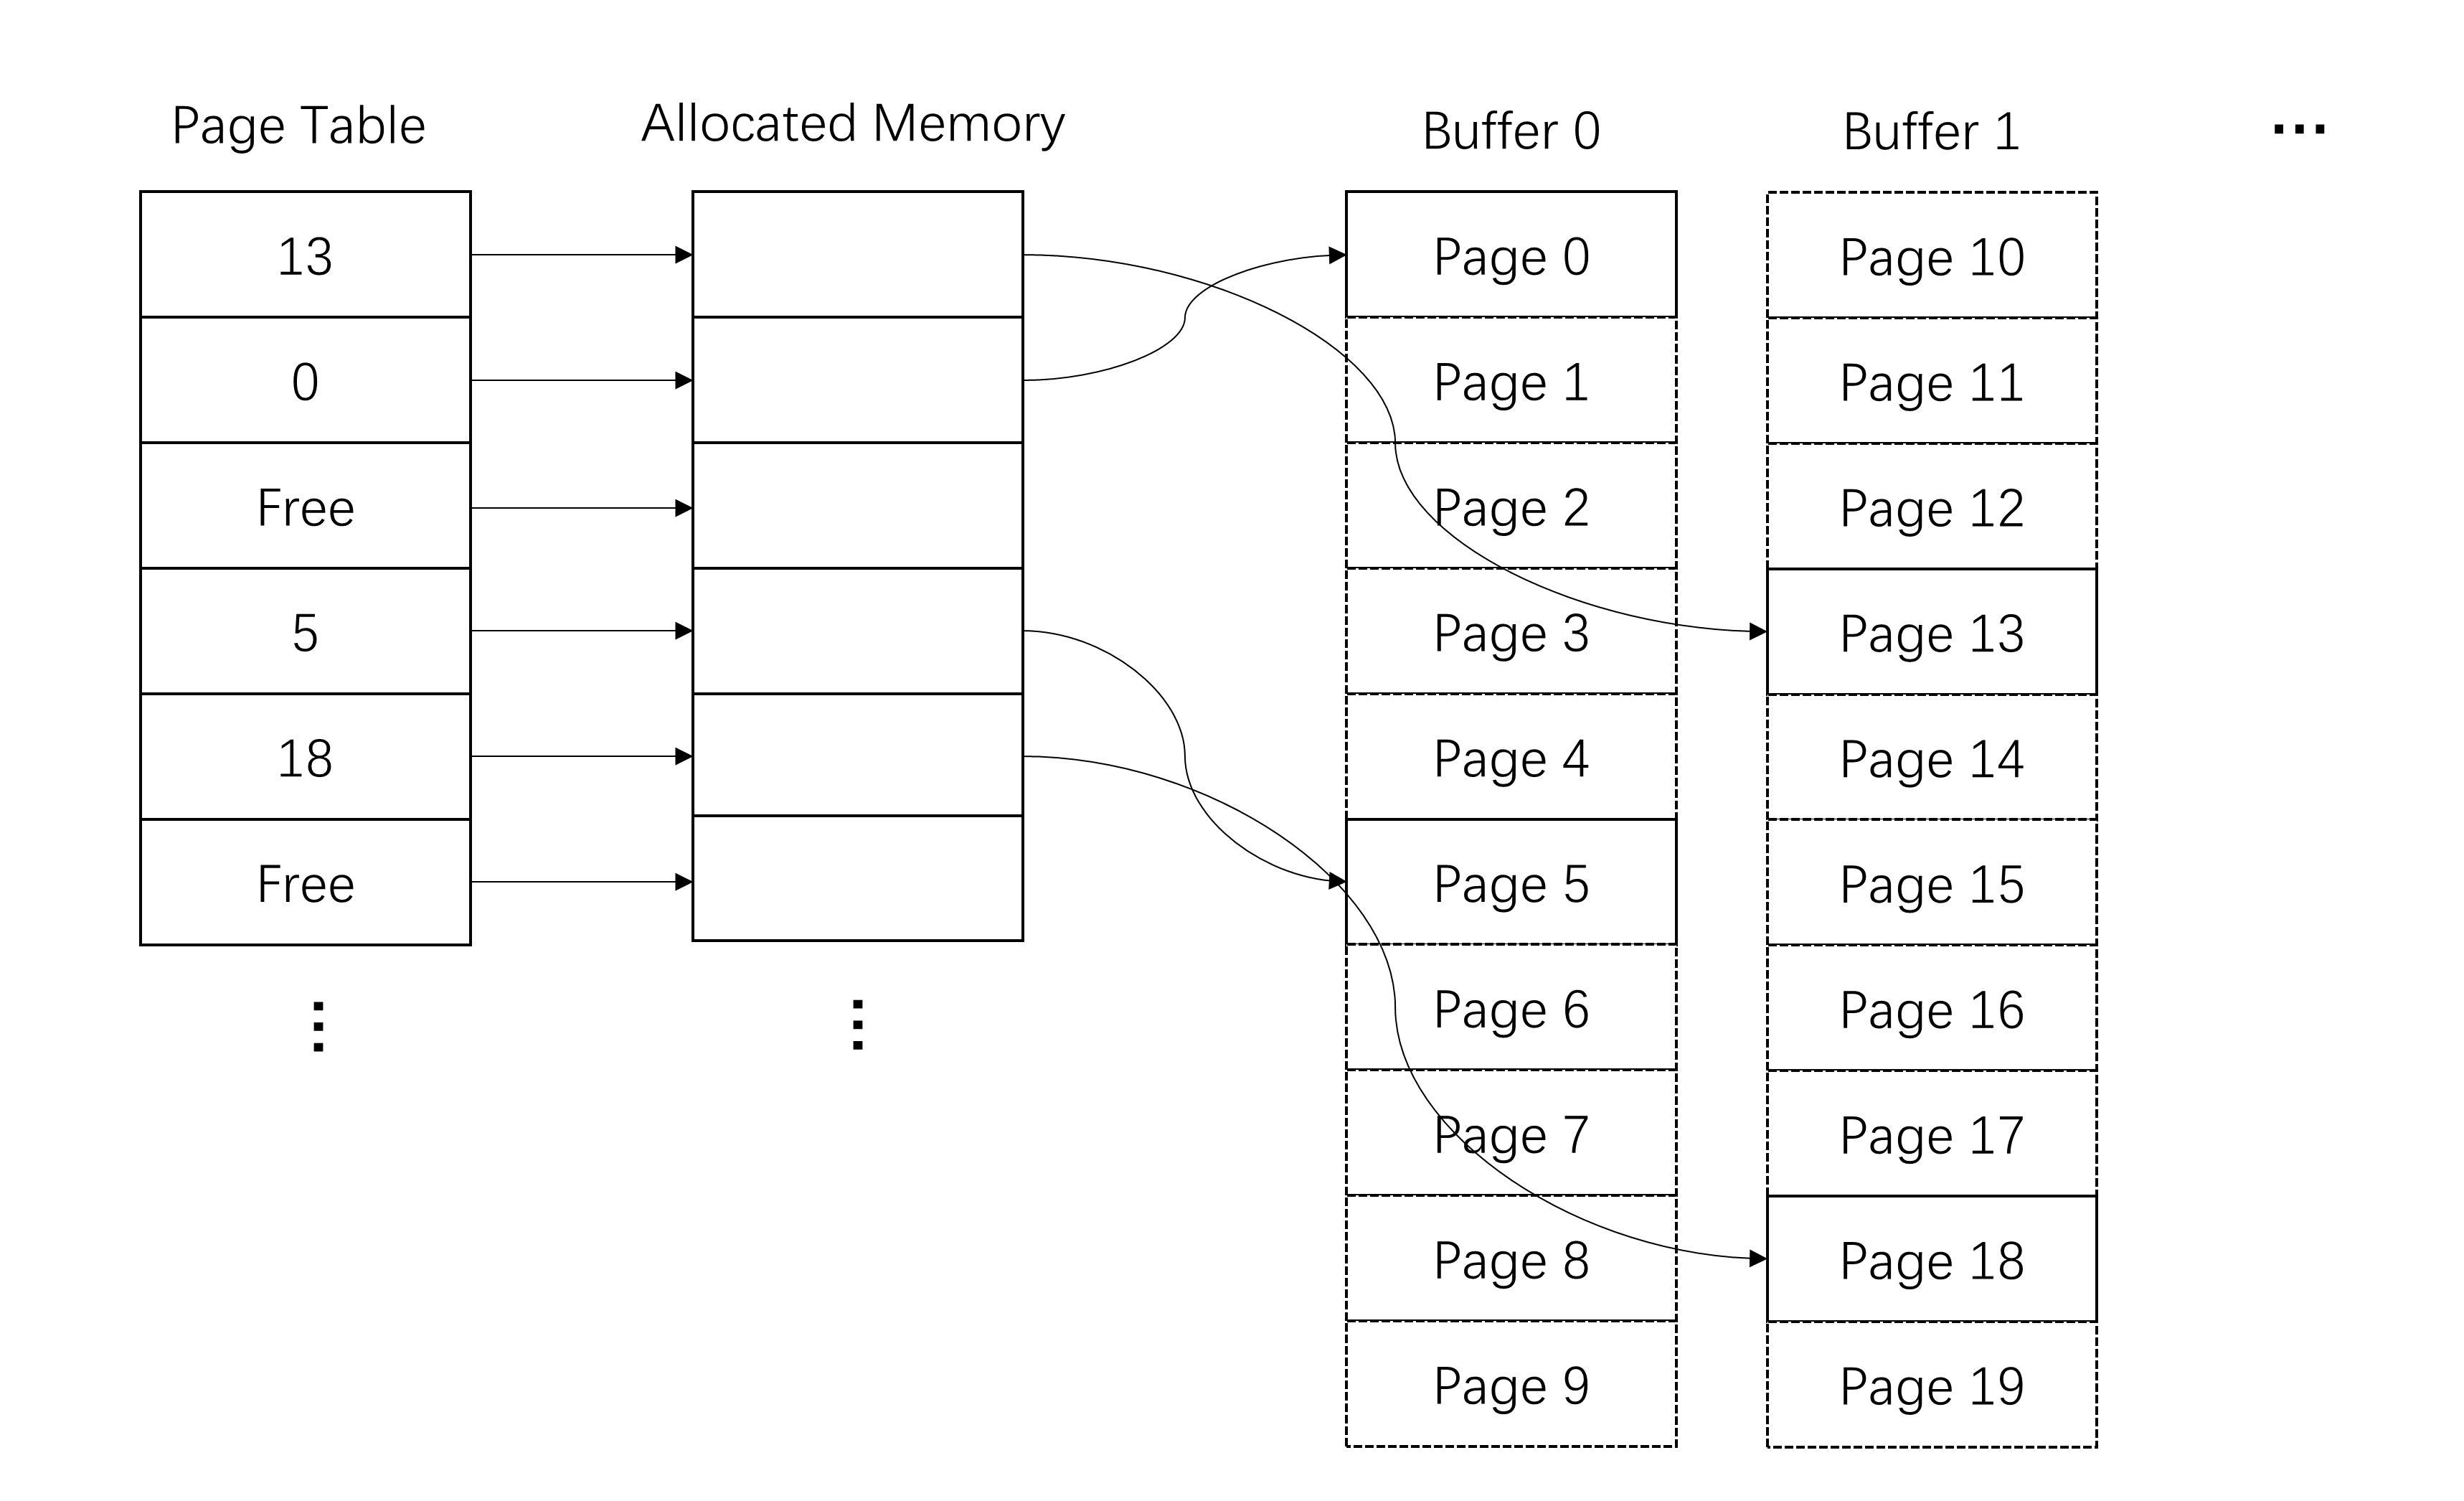
\includegraphics[width=\linewidth]{页表.png}
\caption{\label{fig:page table}页表示意图}
\end{figure}

目前,本项目实现了两种数据页替换策略:一是随机替换策略,在页表已满的情况下,随机选取当前帧未使用的数据页进行换出;二是 LRU(最近最少使用)策略,优先换出最近使用频率最低的数据页。有关两种策略的性能对比将在 \ref{subsec:streaming test} 节中详细讨论。

在极端场景下,若当前视角需要加载的场景数据过多,而页表没有空闲条目且所有数据页都已被当前帧使用,可能导致需要加载的数据页无法换入,从而出现场景“空洞”。为缓解该问题,本项目借鉴拥塞控制(Congestion Control
)思想\cite{Wiki-congestion}:当页表压力过大时,动态提高 \ref{subsec:run-time lod select} 节中所述的 $lod_threshold$,采用更激进的 LOD 选择策略,即便是距离相机较近的物体,也可能选择更为粗糙的 LOD 版本。待页表压力缓解后,系统将逐步恢复原有的 LOD 选择标准。尽管该策略可能在一定程度上降低图像质量,但能有效避免渲染空洞,提升页表管理的鲁棒性与稳定性。

\subsubsection{稀疏资源}

稀疏资源是 Vulkan 1.2 引入的重要扩展,广泛应用于虚拟几何、虚拟纹理(Virtual Texture)等架构\cite{SparseResources}。传统的 Vulkan 资源需完整、连续地绑定至单一显存块,且绑定关系在资源生命周期内不可更改。而稀疏资源突破了这一限制,允许资源分页绑定至多个显存页,并支持动态修改绑定关系,为高效的动态加载机制提供了强有力的支持。关于稀疏资源的详细机制,本文在附录 \ref{appendix:sparse} 中做了进一步阐述。

本项目使用稀疏资源功能构建了一个逻辑上的大型缓冲区(Buffer),用于存储场景的所有几何数据。该缓冲区被划分为若干页,并绑定至多个独立的显存页。由于稀疏资源支持部分区域未绑定显存,因此缓冲区的部分位置并不存在实际数据,如\autoref{fig:page table}所示。

当有新的数据页被换入页表中,CPU 首先提交稀疏绑定命令,将页表位置对应的显存页绑定至缓冲区的目标区域。随后,CPU 再提交数据传输命令,将对应的场景数据复制到缓冲区中。

需要注意的是,Vulkan 对单个缓冲区的大小存在限制。因此,项目中将整个逻辑缓冲区划分成多个大小一致的物理缓冲区,并使用 Vulkan 的 Buffer Device Address 特性进行管理\cite{BDA}。在运行时阶段,为确保安全访问,仅允许网格着色器读取已加载数据的缓冲区区域,避免访问尚未绑定的空白区域。具体地,网格着色器根据当前簇组所在的数据页编号及其在数据页中的偏移量,即可准确计算其对应的缓冲区访问位置。

\subsubsection{异步加载}

为避免数据传输过程阻塞渲染流程,本项目采用了异步加载策略\cite{UnityStreaming}。

本项目创建了独立的传输队列,用于执行数据上传任务,从而避免传输工作与执行绘制命令的图形队列发生竞争。与此同时,针对第 $i$ 帧所需的数据,系统并未在第 $i$ 帧内全部完成加载,而是延后至第 $i{+}1$ 帧渲染之前完成上传。这样可避免图形队列因等待传输队列而发生阻塞,提升了帧间的处理并行度。

理论上,在相机运动较为平稳的情况下,第 $i$ 帧需要的场景数据,大部分与第 $i{-}1$ 帧所需的场景数据重合,\label{subsec:streaming test} 节的实验结果也证明了这一点。因此,即使复用第 $i{-}1$ 帧的几何数据,延迟一帧加载第 $i$ 帧的几何数据,对画面质量的影响微乎其微。但该方法显著提升了系统吞吐率和整体渲染效率,尤其适用于大规模数据场景下的流式加载需求。

\subsection{测试分析报告} \label{subsec:streaming test}

本项目使用了固定的相机轨迹,在 Factory 场景下测试了两种不同换页策略的性能。测试结果如\autoref{tab:swap page}所示。命中概率表示当前帧所需的数据页已在页表中的概率,页表耗时表示每帧维护页表所需的时间,绑定耗时表示每帧执行稀疏绑定操作所需的时间。

\begin{table}[H]
    \caption{\label{tab:swap page}不同换页策略的性能比较}
    \begin{tabularx}{\linewidth}{|X<{\centering}|X<{\centering}|X<{\centering}|X<{\centering}|X<{\centering}|}
        \hline
        换页策略 & 命中概率 & 页表耗时 & 绑定耗时 & 总耗时 \\ \hline
        随机替换 & 99.2\% & 2.86ms & 1.59ms & 4.45ms \\ \hline
        LRU & 99.2\% & 2.67ms & 1.47ms & 4.14ms \\ \hline
    \end{tabularx}
\end{table}

从表格数据可以看出,随机替换和 LRU 策略在命中概率上基本相同,性能差异主要体现在页表和绑定耗时上。LRU 策略在页表维护和绑定过程中的耗时稍低,因此在后续测试中我们选择了性能更优的 LRU 策略。

此外,本项目还对数据页的大小进行了测试,以确定最佳的页大小。在固定页表总容量的前提下,测试了不同数据页大小的性能,结果如\autoref{fig:page size}所示。

\begin{figure}[ht]
    \centering
    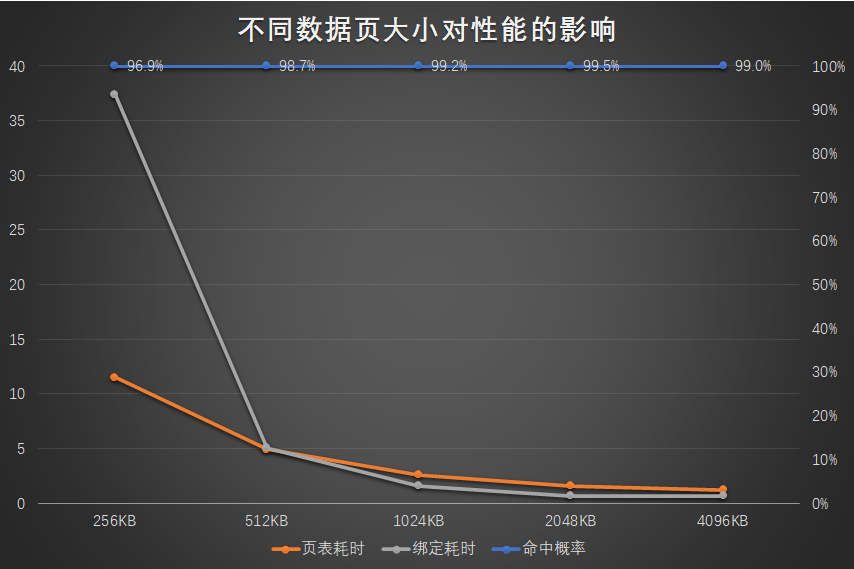
\includegraphics[width=\linewidth]{PageSize.png}
    \caption{\label{fig:page size}不同数据页大小对性能的影响}
\end{figure}

从测试结果可以看出,随着数据页大小的增大,命中概率逐渐提高,同时页表和绑定操作的耗时显著减少。当数据页大小过小时,由于页表容量保持不变,数据页数量较大,导致页表管理的开销上升,进而显著降低了页表的处理速度,同时稀疏绑定所消耗的时间也大幅增加。当数据页大小增大到 4096KB 时,由于页表容量有限,显存利用率下降,页表的压力加大,系统不得不采用更为激进的 LOD 选择策略,这导致了画面质量的明显下降。因此,综合考虑性能和显存利用率,本项目最终选择了 2048KB 作为最优的数据页大小。

\section{项目成果}

\subsection{最终实验结果及分析}

本项目分别对 Sponza、Factory 两个场景进行了最终测试。两个场景的具体参数如\autoref{tab:scene}所示。

\begin{table}[H]
    \caption{\label{tab:scene}测试场景信息}
    \begin{tabularx}{\linewidth}{|X<{\centering}|X<{\centering}|X<{\centering}|}
        \hline
        场景 & 顶点数 & 三角形数 \\ \hline
        Sponza & 190,448 & 262,241 \\ \hline
        Factory & 140,875,512 & 46,958,504 \\ \hline
    \end{tabularx}
\end{table}

在性能测试中,我们分别在启用与未启用 LOD 和流式加载功能的情况下,测量了预处理时间、显存占用、帧时间等关键性能指标。测试结果分别列于\autoref{tab:Sponza data}和\autoref{tab:Factory data}中,最终的运行效果对比如\autoref{fig:Sponza fig}和\autoref{fig:Factory fig}所示。

\begin{table}[H]
    \caption{\label{tab:Sponza data}Sponza 场景运行参数}
    \begin{tabularx}{\linewidth}{|X<{\centering}|X<{\centering}|X<{\centering}|X<{\centering}|X<{\centering}|}
        \hline
        ~ & 预处理时间 & 显存占用 & GPU 时间 & 帧时间 \\ \hline
        不开启 LOD 和流式加载 & 0.2s & 8.0MB & 0.8ms & 1.0ms \\ \hline
        开启 LOD 和流式加载 & 1.8s & 34.5MB & 0.9ms & 1.0ms \\ \hline
    \end{tabularx}
\end{table}

\begin{figure*}[htbp]
    \centering
    % 第一列(远景)
    \begin{subfigure}[b]{0.48\linewidth}
        \centering
        \includegraphics[width=2.9in]{Sponza0.png}
        \caption{不开启 LOD 和流式加载}
    \end{subfigure}%
    \hfill % 确保子图之间有空隙
    % 第二列(中景)
    \begin{subfigure}[b]{0.48\linewidth}
        \centering
        \includegraphics[width=2.9in]{Sponza1.png}
        \caption{开启 LOD 和流式加载}
    \end{subfigure}%
    \caption{Sponza 场景运行效果对比图}
    \vspace{-0.2cm}
    \label{fig:Sponza fig}
\end{figure*}

\begin{table}[H]
    \caption{\label{tab:Factory data}Factory 场景运行参数}
    \begin{tabularx}{\linewidth}{|X<{\centering}|X<{\centering}|X<{\centering}|X<{\centering}|X<{\centering}|}
        \hline
        ~ & 预处理时间 & 显存占用 & GPU 时间 & 帧时间 \\ \hline
        不开启 LOD 和流式加载 & 61s & 5.2GB & 230.3ms & 231.9ms \\ \hline
        开启 LOD 和流式加载 & 1480s & 5.1GB & 38.2ms & 38.5ms \\ \hline
    \end{tabularx}
\end{table}

\begin{figure*}[htbp]
    \centering
    % 第一列(远景)
    \begin{subfigure}[b]{0.48\linewidth}
        \centering
        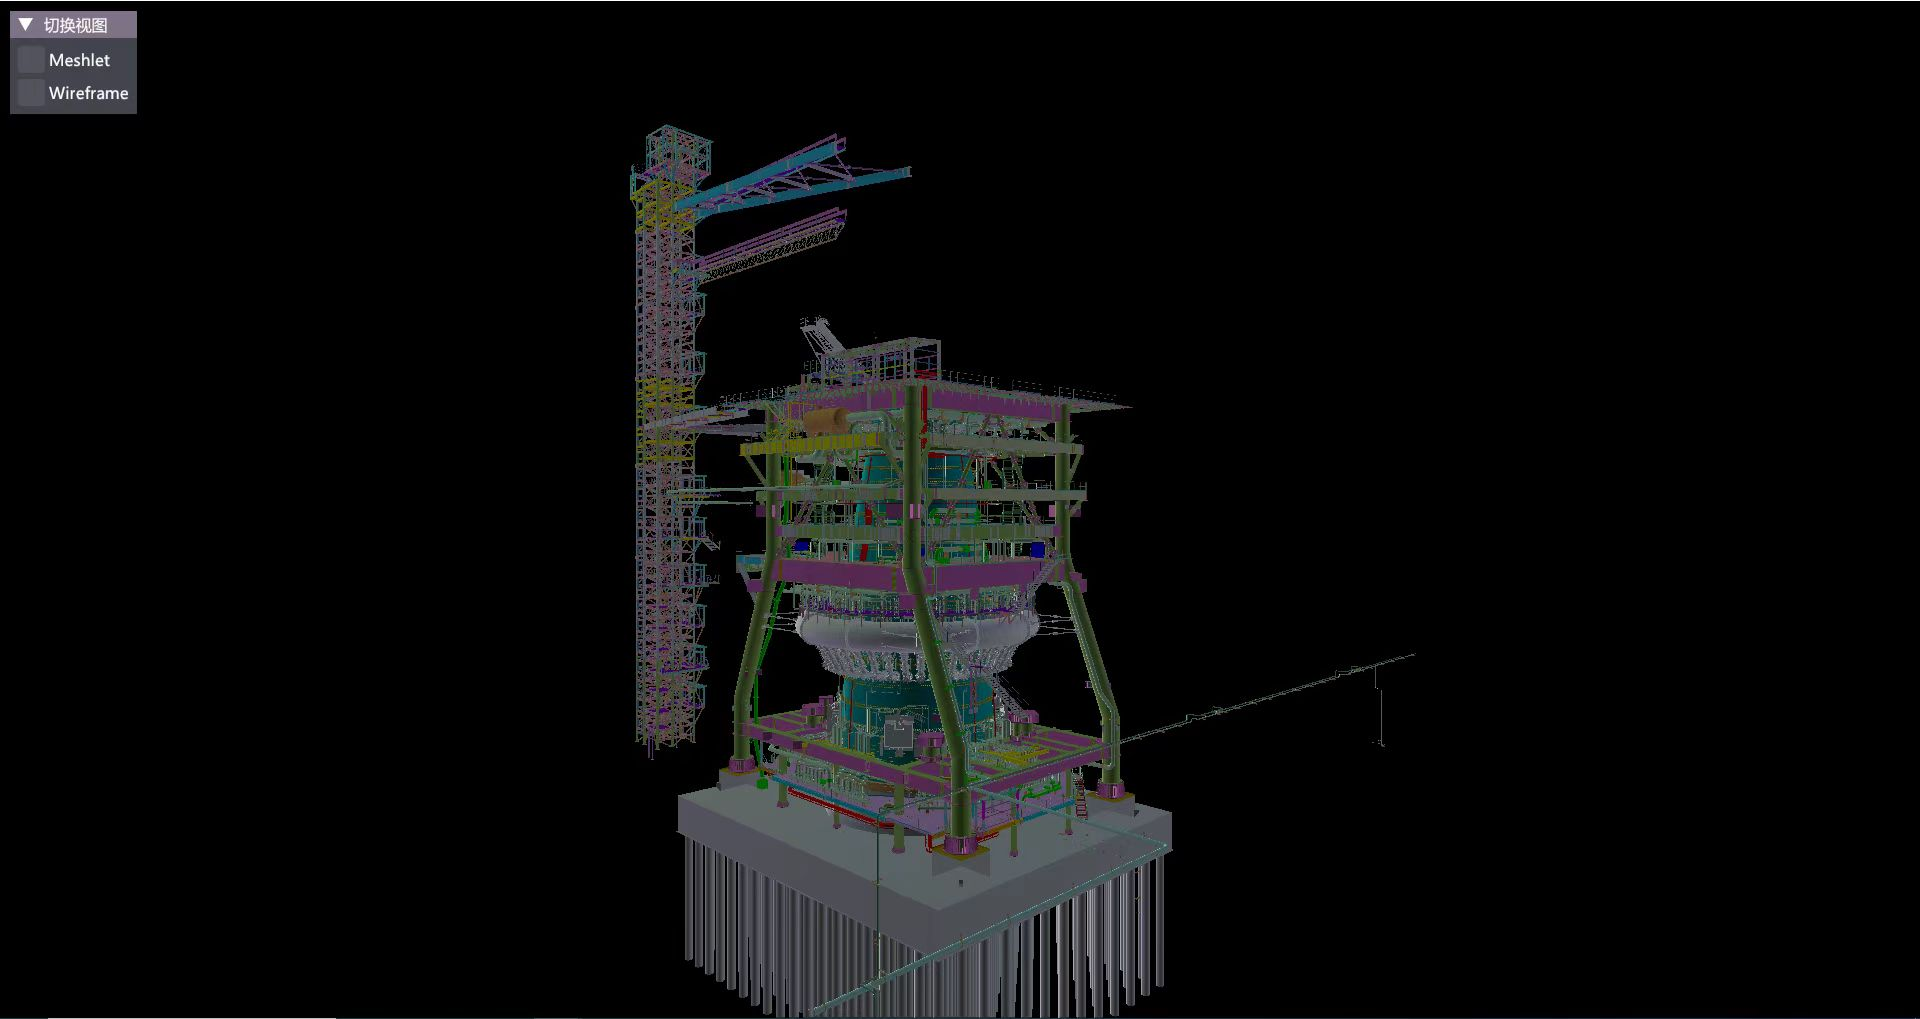
\includegraphics[width=2.9in]{Factory0.jpg}
        \caption{不开启 LOD 和流式加载}
    \end{subfigure}%
    \hfill % 确保子图之间有空隙
    % 第二列(中景)
    \begin{subfigure}[b]{0.48\linewidth}
        \centering
        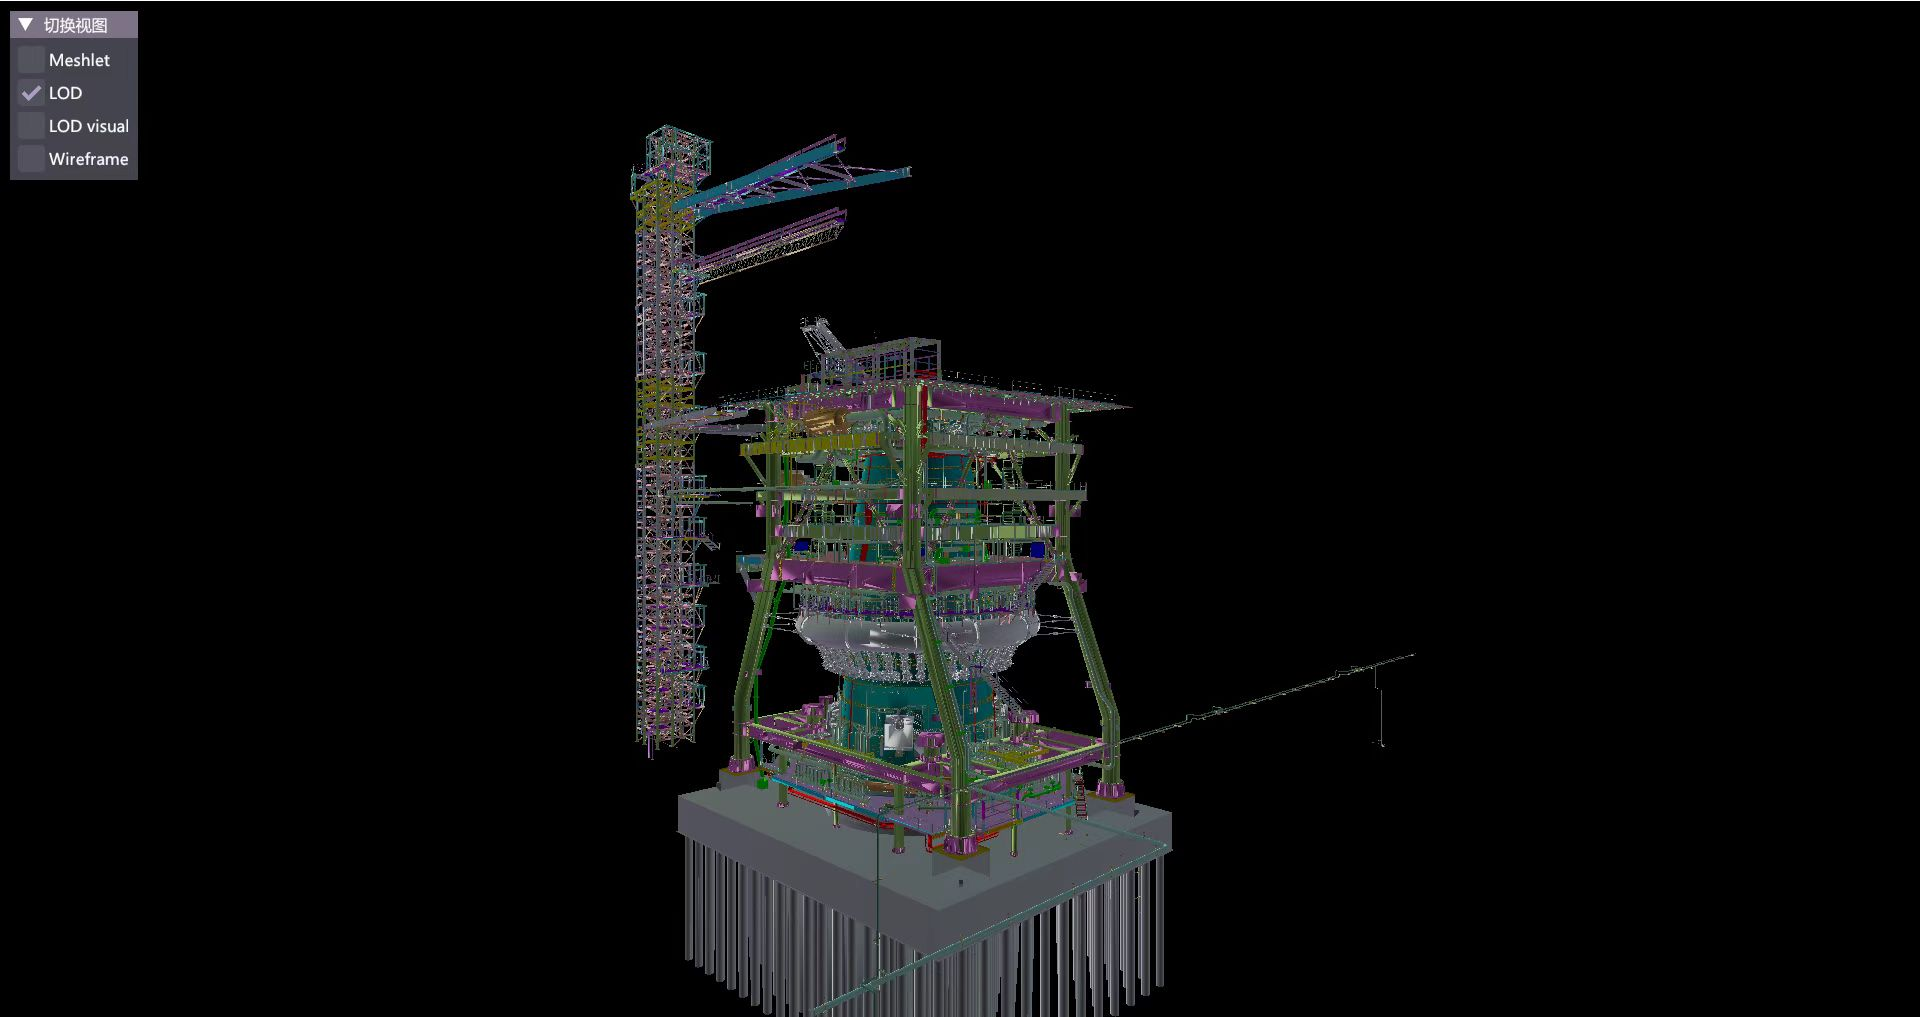
\includegraphics[width=2.9in]{Factory1.jpg}
        \caption{开启 LOD 和流式加载}
    \end{subfigure}%
    \caption{Factory 场景运行效果对比图}
    \vspace{-0.2cm}
    \label{fig:Factory fig}
\end{figure*}

从实验结果来看,对于简单场景(如 Sponza),LOD 与流式加载带来的性能收益较为有限;而在复杂工业场景(如 Factory)中,这些优化措施显著提升了渲染性能。帧率从不足 5 FPS 提升至约 25 FPS,实现了接近 5 倍的加速,基本满足实时交互需求。同时可见,开启流式加载后 GPU 时间与整体帧时间相近,说明虽然存在 CPU 与 GPU 之间的数据交互,但并未造成明显的 CPU 负担,系统整体处于良好的负载均衡状态。

不过,画面质量上仍存在一些问题。如\autoref{fig:Factory fig}所示,开启 LOD 后画面出现明显走样现象。初步分析是预处理过程中的顶点合并操作未充分考虑法向量因素,导致法向量精度下降,进而在光照计算中出现较大误差。后续需进一步改进法向量处理策略,提升画面质量。

与此同时,启用 LOD 与流式加载功能后,预处理时间显著增加。对于千万级多边形的模型,预处理时间可达 25 分钟左右。为避免用户在每次使用引擎时都重复执行预处理过程,本项目将预处理后的数据通过可持久化存储保存至磁盘中\cite{cereal}。此举不仅显著提升了系统的启动速度,还保证了预处理结果的一致性,方便在后续运行中快速加载和复用。

\subsection{工作总结}

综上所述,本项目在深入理解 Nanite 核心思想的基础上,结合 Vulkan 这一现代图形 API 和现有引擎架构,成功实现了基于簇的 GPU 驱动渲染管线。通过引入流式加载机制,即使是在场景数据体量远超显存容量的情况下,系统依然可以导入和渲染。在 LOD 技术的加持下,系统能够动态调整渲染精度,兼顾画质与性能,显著提升了整体渲染效率。与传统的 CPU 驱动渲染管线相比,本项目在大规模工业场景中的性能提升最高可达约 5 倍。

总体而言,本项目为大规模高精度工业场景的实时渲染提供了切实可行的技术路径,并为今后在该领域的进一步研究与应用奠定了坚实基础。

\subsection{未来展望}

尽管本项目在大规模工业场景的实时渲染方面已取得初步成果,但距离实际工程应用仍存在一定差距。未来的改进方向主要包括:

\begin{itemize}
    \item \textbf{添加阴影支持}:由于改动了场景的存储结构,原引擎的阴影算法无法直接复用,需要自行设计一种适配当前场景结构的阴影算法。可参考虚幻引擎中的虚拟阴影贴图(Virtual Shadow Map, VSM)方案\cite{VSM},并加以适当改动,以实现高效的阴影算法。

    \item \textbf{实现高效的遮挡剔除}:目前管线只支持视锥剔除和圆锥剔除,缺乏高效的遮挡剔除(Occlusion Culling)机制。未来可引入遮挡查询技术,剔除更多不需要渲染的多边形,进一步释放性能\cite{coorg1997};

    \item \textbf{支持多材质系统}:当前渲染管线只支持单一材质的渲染。未来可以参考延迟材质(Deferred Material)的思想,实现一个可见性缓冲区(Visibility Buffer),来支持多个材质的同时渲染\cite{burns2013};

    \item \textbf{实现场景数据编码与解码}:在预处理阶段对场景数据进行编码,进一步压缩场景大小,可以显著降低显存、内存乃至磁盘空间的使用\cite{Mlakar2024}。同时,还需在 GPU 上实现高效的解码算法,保证渲染性能不受影响。
\end{itemize}

上述改进将进一步提升本项目在大规模工业场景中的实时渲染能力和视觉表现力,为其在工程可视化、数字孪生等实际应用中奠定技术基础。